\documentclass[11pt]{article}

\usepackage[a4paper,margin=25mm,headheight=14pt]{geometry}
\usepackage{fontspec}
\usepackage{unicode-math}
\setmainfont{Times New Roman}
\setsansfont{Arial}
\setmonofont{Menlo}
\setmathfont{STIX Two Math}
\usepackage{microtype}
\usepackage{amsmath,amsthm,mathtools}
\usepackage{booktabs,tabularx,longtable,array}
\usepackage{enumitem}
\usepackage{xcolor}
\usepackage{tikz}
\usetikzlibrary{arrows.meta,positioning,fit,calc}
\usepackage{fancyhdr}
\usepackage{hyperref}

\definecolor{navy}{HTML}{17365D}
\definecolor{blue}{HTML}{2F5597}
\definecolor{lightblue}{HTML}{EAF1F8}
\definecolor{deepred}{HTML}{8B1E2D}
\definecolor{graytext}{HTML}{4A4A4A}
\hypersetup{colorlinks=true,linkcolor=navy,citecolor=deepred,urlcolor=blue,pdfauthor={Satoru Watanabe},pdftitle={Subjectivity Intersection Mathematics: A Pointed-Braid Source for Quantum History, Lorentzian Geometry, and Reciprocal Backreaction}}

\newtheorem{theorem}{Theorem}[section]
\newtheorem{proposition}[theorem]{Proposition}
\newtheorem{lemma}[theorem]{Lemma}
\newtheorem{corollary}[theorem]{Corollary}
\theoremstyle{definition}
\newtheorem{definition}[theorem]{Definition}
\newtheorem{assumption}[theorem]{Assumption}
\theoremstyle{remark}
\newtheorem{remark}[theorem]{Remark}

\newcommand{\cH}{\mathcal{H}}
\newcommand{\cA}{\mathcal{A}}
\newcommand{\cC}{\mathcal{C}}
\newcommand{\Tr}{\operatorname{Tr}}
\newcommand{\id}{\mathbf{1}}
\newcommand{\dd}{\mathrm{d}}
\newcommand{\ad}{\operatorname{ad}}
\newcommand{\Ric}{\operatorname{Ric}}
\newcommand{\Span}{\operatorname{span}}
\newcommand{\rank}{\operatorname{rank}}
\newcommand{\Ker}{\operatorname{ker}}
\newcommand{\im}{\operatorname{im}}
\newcommand{\Lie}{\mathcal{L}}
\newcommand{\RC}{\mathcal{R}_{C}}

\pagestyle{fancy}
\fancyhf{}
\fancyhead[L]{\small\color{graytext}Pointed-braid quantum, Lorentz, and backreaction system}
\fancyhead[R]{\small\color{graytext}Working preprint v0.8}
\fancyfoot[C]{\thepage}

\setlength{\parindent}{0pt}
\setlength{\parskip}{0.65em}
\setlist{nosep,leftmargin=1.5em}

\title{\vspace{-1.2cm}\textbf{Subjectivity Intersection Mathematics:}\\[0.18em]\textbf{A Pointed-Braid Source for Quantum History, Lorentzian Geometry, and Reciprocal Backreaction}\\[0.35em]\Large Infinite algebraic completion, rank-ten metric readout, and a fail-closed stress gate}
\author{Satoru Watanabe\\\small Subjectivity Intersection Emergence Lab (SIEL)}
\date{Working preprint v0.8 --- 15 September 2026}

\begin{document}
\maketitle

\begin{center}
\fcolorbox{navy}{lightblue}{\parbox{0.91\linewidth}{\small
\textbf{Status.} This is a working theoretical preprint. Version 0.8 preserves the scope corrections of v0.7 and adds two completed mathematical advances. First, the all-finite-stage matrix tower has a standard type-$5^\infty$ UHF $C^*$-completion with a unique trace, a compatible conditional expectation to the $25\times25$ base algebra, a bounded extension of the selected rank-ten metric readout, an explicit uncountable compact family of states, and finite-supported Braid automorphisms. This is an infinite-dimensional algebraic and state-space completion, not a derivation of continuous spacetime, physical time, or infinite-mode QFT. Second, the post-UB610 stress analysis reaches UB622: it constructs the finite-prefix Wightman Cauchy kernel, proves the actual matrix-SLE ultraviolet principal coefficient and exact complete $SU(2)$ shell count, controls the finite-shell matrix remainder, and reduces the unresolved global reference contribution to one explicit subtract-first inequality. The complete smooth finite stress, fixed coupling, conserved ten-tensor history, cutoff-uniform field limit, general $3+1$ evolution, Braid necessity, and natural validation remain open. This version is not peer reviewed and does not establish completed quantum gravity, empirical general relativity, SIC/O3 ontology, subjectivity, or consciousness.}}
\end{center}

\begin{abstract}
We construct a typed system in which quantum history, a section-free Lorentzian event carrier, a nonterminal algebraic source tower, and reciprocal geometric response share one actual pointed-braid source. A central Braid-Casimir generator supplies an exact parameterized Yang--Baxter path and finite-time $*$-automorphisms. Under explicit Lorentz-completion, homogeneous PBM--BIX, state-selection, material-current, and reciprocal-response assumptions, the same source data enter a conditional semiclassical gravity system.

The finite source is not a terminal carrier. One fixed $25\times25$ crossing generates $\cA_n=M_{5^n}(\mathbb C)$ at every finite stage. Version 0.8 retains an all-finite-stage family of normalized conditional expectations and typed response maps satisfying exact recovery, nonzero marked-boundary response, and bilateral re-entry into one fixed $87$-coordinate PBM--BIX response system. The tower is detected by response history rather than embedded into $F_{87}$.

We further take the standard norm completion
\begin{equation*}
  \cA_\infty=\varinjlim_n\bigl(M_{5^n}(\mathbb C),X\mapsto X\otimes\id_5\bigr).
\end{equation*}
It is the unital type-$5^\infty$ UHF algebra. The compatible normalized traces induce its unique tracial state, tail tracing extends to a norm-one conditional expectation $E_{2,\infty}:\cA_\infty\to M_{25}(\mathbb C)$, and the selected rank-ten linear metric map extends boundedly through $E_{2,\infty}^{\oplus4}$. An explicit product-state family embeds $[0,1]$ continuously into the state space, while each finite-supported Braid word acts by an inner automorphism. This closes an infinite algebraic carrier and a mathematical state continuum, not physical spacetime, continuous physical time, or an infinite-mode field theory. The construction still depends on normalized-trace neutrality; neither the number 87, the UHF completion, nor its trace is uniquely Braid-specific.

For the quantum state, a fixed no-occupation-fit $G_1$-clock state-of-low-energy rule defines a unique target-blind parametric matrix-SLE family on the recorded compact extrinsic-curvature box. The family is qualitatively Hadamard uniformly in the parameter. More strongly, every finite local symbol coefficient of the same-operator $W-H_{\mathrm{ps}}$ stress kernel, including four fixed-chart derivatives, cancels before interval absolute values are taken. This closes the ultraviolet subtraction problem but not the nonlocal smooth finite coincidence limit.

For semiclassical backreaction, an exact nonzero small-coupling constraint branch exists. On the frozen $l\le16$ prefix, the energy response and cubic flux response form a nonzero four-constraint Jacobian; the flux block has rank three, condition number approximately $5.23$, and its complete all-time-order finite-prefix remainder lies below $10^{-234}$ and far below the fixed momentum-face budget. These facts do not establish the target coupling $\alpha=1$, because the aggregate smooth $W-H_{\mathrm{ps}}$ tail remains unresolved.

The fail-closed tail audit is itself informative. A local Hadamard germ has no canonical global Peter--Weyl blocks. The tested unsigned positive-$\tau$ Abel envelopes are non-discriminating: their narrowest energy half-width exceeds the fixed face margin by $9.96\times10^{11}$, and their flux half-width exceeds its budget by $3.20\times10^9$. This is enclosure slack, not a physical lower bound and not a refutation of the candidate. UB610 carries the actual finite prefix into the signed-local scheme. UB611--UB622 then replace the missing global reconstruction by a finite covariant coincidence-jet contract, construct the propagated finite-prefix Wightman Cauchy kernel, prove the actual matrix-SLE ultraviolet mixing coefficient and exact complete $SU(2)$ shell count, obtain a dimension-free finite-shell remainder bound, and reduce the remaining global adiabatic-reference obstruction to one explicit subtract-first inequality. That inequality is not proved here, so no fixed-coupling stress root follows.

A conditional local-existence and Ward--Bianchi propagation schema holds for a fixed finite homogeneous Galerkin BIX Einstein--Klein--Gordon system, provided the complete same-scheme conserved ten-tensor callback is supplied. Cutoff-uniform infinite-mode existence, general inhomogeneous $3+1$ evolution, low-energy recovery from Braid rather than assumption, Braid necessity, and natural-data validation remain open. The result is therefore a mathematically explicit quantum-gravity candidate architecture, not a completed or empirically validated unified physical theory.
\end{abstract}

\noindent\textbf{Keywords:} braid group; Yang--Baxter coherence; inductive matrix tower; quantum geometry; Lorentzian metric; Hadamard state; state of low energy; quantum dynamical semigroup; backreaction; relational observable.

\section{Problem and claim}

Many quantum--geometry constructions begin with a quantum model and a spacetime model that have independent state spaces, independent clocks, or independently normalized energies. A coupling term can then connect them, but the coupling alone does not show that they arise from one mathematical source. The question addressed here is narrower and stricter:

\begin{quote}
Can the quantum history, the initial Lorentzian geometry, the relational component that mediates their coupling, and the subsequent backreaction be placed on one source-derived object without duplicating the source or selecting one braid presentation as absolute?
\end{quote}

The answer is conditional but constructive. The central result is a local composition theorem for a fixed finite source. Its content is stronger than compatibility of two separately specified models: all source readouts come from one joint state, the source Hamiltonian is counted once, the initial metric is generated from the same reduced state that carries the quantum history, and the coupled state and metric then evolve in one local initial-value problem.

The result also has strict boundaries. Braid relations do not by themselves select four dimensions, the physical clock soldering, the reflection coefficient used to obtain Lorentz signature, the relative gravitational source law, or the absolute units. The construction therefore separates four layers:

\begin{enumerate}
\item exact finite algebra and exact rational certificates;
\item conditional mathematical composition under explicit bridge assumptions;
\item an unadopted finite-source physical model with an operational discriminator;
\item ontological interpretation, which is not proved here.
\end{enumerate}

Version 0.8 continues to separate two completion targets. The \emph{effective U4 target} asks whether one explicitly assumed compact homogeneous QFT--geometry model closes on a controlled interval and survives a frozen natural-data test. The stronger \emph{Braid-origin target} additionally requires the real continuum, the physical state rule, the microscopic dissipative sector, and the tower-to-response anchor to arise without stagewise fitting from the finite pointed-braid datum. Progress toward the first target must not be reported as completion of the second.

Classical braid groups and Yang--Baxter consistency provide the mathematical background for the path equivalences used below \cite{artin1947,yang1967,lamberadford1997}. The direct source theorem is Watanabe's pointed-unitary-braid result: it proves canonical all-finite-orders endpoint overlaps, bilateral positive contractions, pointed-unitary covariance, and compatibility with the declared shuffled tensor law \cite{watanabe2026braid}. The present paper uses that theorem as its Braid foundation and does not strengthen its scope. Local covariance and the initial-value structure of general relativity supply comparison standards for the field-theoretic and geometric parts \cite{brunetti2003,choquet2008}. The construction is not presented as a replacement for those frameworks.

\section{The fixed pointed-braid source}

\subsection{One source state and its endpoint readouts}

Let
\begin{equation}
  \cH_{\mathrm{src}}=\cH_A\otimes\cH_B,
  \qquad \cH_A=\cH_B=\mathbb{C}^{125}.
\end{equation}
The actual finite source state used throughout the composition is
\begin{equation}\label{eq:gamma0}
  \Gamma_0=\frac{100\id+D\otimes D}{1{,}562{,}500},
  \qquad \Tr D=0,\qquad \Tr(D^2)=216.
\end{equation}
It is normalized and has maximally mixed endpoint marginals,
\begin{equation}
  \Gamma_A=\Tr_B\Gamma_0=\frac{\id_{125}}{125},
  \qquad
  \Gamma_B=\Tr_A\Gamma_0=\frac{\id_{125}}{125}.
\end{equation}

The full source package also contains the original Hamiltonian $H$, a fixed endpoint split, the cup mark $M_0$, insertion data, polar data, and selected graded generators. These objects are transported together. None is reconstructed from a scalar summary of the state.

The coupled system has one joint state $\Sigma(t)$ on
\begin{equation}
  \cH_{\mathrm{src}}\otimes\cH_F,
  \qquad \Sigma(0)=\Gamma_0\otimes\rho_F,
  \qquad \Tr\rho_F=1.
\end{equation}
The time-dependent source state is only the readout
\begin{equation}\label{eq:reduced}
  \Gamma(t)=\Tr_F\Sigma(t).
\end{equation}
Thus $\Gamma$ is not a second dynamical copy.

\subsection{The endpoint-invisible correlation carrier}

For any normalized bipartite state $\Gamma$, define
\begin{equation}\label{eq:corr}
  c_\Gamma=\Gamma-\Gamma_A\otimes\Gamma_B,
  \qquad
  \cC_{\mathrm{corr}}=\Ker\Tr_A\cap\Ker\Tr_B
\end{equation}
inside the real vector space of trace-zero Hermitian joint variations. For the actual state,
\begin{equation}
  c_0=\frac{D\otimes D}{1{,}562{,}500},
  \qquad
  \Tr(c_0^2)=\frac{216^2}{1{,}562{,}500^2}>0.
\end{equation}

Let $p=(\Tr_B,\Tr_A)$. The inclusion
$\iota:\cC_{\mathrm{corr}}\hookrightarrow\mathrm{Herm}_0(\cH_A\otimes\cH_B)$
is the categorical kernel of $p$ in the declared finite-dimensional real-linear category: every $T:Z\to\mathrm{Herm}_0$ satisfying $pT=0$ factors uniquely through $\iota$. Moreover, every normalized joint state has the unique decomposition in Eq.~\eqref{eq:corr}.

This universal property is elementary finite bipartite mathematics; it is not uniquely braid-specific. The source-specific content enters through the actual state, cup, operators, and their simultaneous transport. A matched control with unchanged endpoint marginals but a rotated right correlation factor changes a fixed cup response by the exact amount $62/48{,}828{,}125$. Therefore that joint response cannot factor through either endpoint marginal alone. This is an operational nonfactorization result, not an ontological identification of $c_\Gamma$.

\subsection{Typed braid descent}

Let $\mathsf{Cross}$ be the free typed crossing groupoid generated by the allowed elementary crossings and let $\mathsf{Braid}$ be its quotient by Yang--Baxter, remote-commutation, inverse, and unit relations. A typed output functor $F$ includes the labelled source history, the joint source-field evolution, the energy ledger, the relation mark, initial soldering, the field, and the local geometric problem.

\begin{proposition}[Typed descent criterion]\label{prop:descent}
$F$ factors uniquely through $\mathsf{Braid}$ if and only if it maps both sides of every generating relation to the same typed output.
\end{proposition}

\begin{proof}
This is the quotient universal property. Necessity follows because equivalent words have one image in the quotient. Sufficiency follows because equality on generating relations makes $F$ constant on the generated congruence, hence defines a unique functor on the quotient.
\end{proof}

The actual even typed source satisfies the required relations in the fixed-finite scope. A non-Yang--Baxter unitary control fails: for a retained label $p=|000\rangle\langle000|$, the two relation words produce orthogonal projector images and
\begin{equation}
  \Delta_p=\|\operatorname{Ad}_{W_L}(p)-\operatorname{Ad}_{W_R}(p)\|_{\mathrm{HS}}^2=2.
\end{equation}
The ordinary flip also satisfies Yang--Baxter, so descent proves a coherence role for braid structure but not uniqueness of the concrete raw representation.

The scope of Proposition~\ref{prop:descent} is a finite typed congruence quotient. It is not a theorem about arbitrary measurable or stochastic response quotients. If a later construction descends a Markov kernel through a response-equivalence relation, the quotient pushforward must be constant on every source equivalence class, and the measurable quotient structure must be supplied explicitly. Even when each adjacent kernel descends, pairwise descent alone does not imply that direct transport agrees with transport along every composite path; global path independence requires a separate coherence condition.

\section{Initial Lorentzian geometry from the same source}

\subsection{A four-plane and ten independent metric directions}

The graded-greedy covariance-cone rule begins with the distinguished grade-one Hamiltonian generator and repeatedly adjoins the least higher grade whose unordered pair sums remain distinct and whose required source pivots are nonzero and untruncated. Stopping at four directions gives
\begin{equation}
  (1,2,4,8),\qquad
  V=\Span_{\mathbb{R}}\{H,U_2,U_4,U_8\}.
\end{equation}
The ten unordered pair sums are
\begin{equation}
  2,3,5,9,4,6,10,8,12,16,
\end{equation}
all distinct. An exact triangular-minor certificate gives rank ten for the metric Jacobian. With source grade $m=3$ and declared finite bound $J=83$, every selected pivot is untruncated because $m+16\le J$.

Four directions are required here because the target is a symmetric $4\times4$ tensor with ten components. This stopping rule is an explicit construction choice; it is not a theorem that bare braid relations force four spacetime dimensions.

\subsection{Covariance cone and Lorentz signature}

For selected source generators $G_a$ and a clock operator $O_0$, define the centered covariance tensor
\begin{equation}
  K_{ab}=\Tr\Gamma\,\Delta Z_a\Delta Z_b,
  \qquad h_{ab}=\Re K(G_a,G_b),
\end{equation}
and clock response
\begin{equation}
  v_a=-2\Im K(G_a,O_0).
\end{equation}
At the actual base point, the exact response is
\begin{equation}
  v=(17/4,0,0,0).
\end{equation}
Normalize
\begin{equation}
  \theta=\frac{v}{\sqrt{v^{\mathsf T}h^{-1}v}}
\end{equation}
and impose the declared clock reflection
\begin{equation}\label{eq:lorentzmetric}
  g_0=h-2\,\theta\otimes\theta.
\end{equation}
Then $g_0$ has signature $(-,+,+,+)$, and
\begin{equation}
  K_{\mathrm{cov}}=\{x:\theta(x)\ge0,\ g_0(x,x)\le0\}
\end{equation}
is closed, convex, pointed, and full dimensional. Its $\theta=1$ section is a nondegenerate solid $h$-ellipsoid in $\Ker\theta$.

Equation~\eqref{eq:lorentzmetric} is a source-internal Lorentz construction. Equality with a separately measured natural light cone is not proved. The geometry map will be denoted $G$, so the typed initial creation identity is
\begin{equation}\label{eq:creation}
  g_0=G(\Gamma_0)=G(\Tr_F\Sigma_0).
\end{equation}

\section{One quantum--geometry evolution}

\subsection{Clock and energy soldering}

Three clock descriptions occur: the original $H$-evolution parameter $t$, the source covector $\theta$, and a material scalar $T$ in the local field system. Their physical identity is not a consequence of the braid relations. We impose the explicit noncircular soldering condition along one timelike anchor $\gamma$,
\begin{equation}\label{eq:clock}
  T(\gamma(t))=t,\qquad u(T)=1,\qquad \dd T\parallel\theta\quad\text{initially}.
\end{equation}

The source energy is counted once:
\begin{equation}\label{eq:energy}
  e(\Sigma)=\frac12\Tr\!\left[\Sigma(H\otimes\id_F)\right]
  =\frac12\Tr(\Gamma H).
\end{equation}
For vanishing coupling, the full source algebra follows the original free history
\begin{equation}
  \alpha_t^H(a)=e^{itH}a e^{-itH}.
\end{equation}
At nonzero coupling, the joint history is not identified with $\alpha_t^H$ on source words that do not commute with $H$.

\subsection{A common interaction and relative stress}

The retained local linear interaction is
\begin{equation}\label{eq:interaction}
  S_{\mathrm{int}}=-\lambda\int \chi(T)\,H\otimes\phi\;\dd T\wedge N,
\end{equation}
where $N$ is the local current three-form and $\chi$ is fixed in advance. Only the abelian charge algebra $C^*(H)$ enters spacelike local densities; the full noncommutative source remains on one timelike defect. The interaction commutes with $H\otimes\id_F$, preserving Eq.~\eqref{eq:energy} and the $H$-sector populations. On a fixed smooth background, the spectral sectors of $H$ give retarded affine scalar shifts and a controlled-Weyl joint propagator.

The geometric source is relative. For an advance-fixed reference state and the same metric and prescription, define
\begin{equation}
  \Delta T_\phi[g;\Sigma,\Sigma_{\mathrm{ref}}]
  =T_\phi[g,\Sigma]-T_\phi[g,\Sigma_{\mathrm{ref}}].
\end{equation}
Common state-independent geometric counterterms cancel in the difference. The proposed finite-model field equation is
\begin{equation}\label{eq:gravity}
  E_c[g]=G[g]+\Lambda g
  =\kappa\left(\Delta T_\phi+T_{\mathrm{mat}}+2\Pi\right).
\end{equation}
This is the \emph{Intersection-Relative Gravity} working law. It is a constitutive proposal, not a derived absolute semiclassical Einstein equation. Standard semiclassical gravity also couples quantum stress to classical geometry, but the well-definedness, renormalization, and backreaction problem is delicate \cite{hollandswald2001,pinamontisiemssen2021,meda2026}.

\subsection{Relation polarization and reciprocal backreaction}

The cup-marked relation selects an energy-tangent source direction $\Xi_C$. The geometry differential and spatial projection define
\begin{equation}\label{eq:dc}
  d_C=P_{\mathrm{sp}}DG\,\Xi_C.
\end{equation}
At the actual base point, one exact projected coordinate lies in the strictly negative interval
\begin{equation}
  -\frac{1127}{50{,}000{,}000{,}000}
  \le Dq[\Xi_C]\le
  -\frac{563}{25{,}000{,}000{,}000},
\end{equation}
so $d_C\ne0$. The relation enters as a zeroth-order target shift,
\begin{align}
  m_{\mathrm{sp}}^{\mathrm{RP}}
  &=P_{\mathrm{sp}}(w-DG\,X_H)-d_C,\\
  \frac{8K}{\rho}D_u^P\Pi+\Pi
  &=-K m_{\mathrm{sp}}^{\mathrm{RP}}.\label{eq:rp}
\end{align}
The source row retains the original intrinsic generator,
\begin{equation}
  D_u^B\Gamma=(I-P_H)X_H+R_E\Lie_u g,
\end{equation}
and the relation mark is transported by $D_uM=0$. On the regular patch, $d_C$ depends smoothly and algebraically on $(\Gamma,g,M)$. Consequently the feedback loop is
\begin{equation}\label{eq:loop}
  (M,\Gamma)\longrightarrow d_C\longrightarrow\Pi
  \longrightarrow g\longrightarrow\Gamma.
\end{equation}
The coefficient of $d_C$ in Eq.~\eqref{eq:rp} is a bold constitutive choice. It is not uniquely selected by the braid relations.

\subsection{Emergent-then-autonomous geometry}

The equality in Eq.~\eqref{eq:creation} is imposed only at the creation/soldering datum. Afterwards $g$ and $\Sigma$ are distinct state variables of the same coupled system. Requiring $g=G(\Tr_F\Sigma)$ at every time would both reduce geometry to an algebraic readout and conflict with the retained sector structure. The post-creation state space therefore realizes provenance without permanent algebraic identity.

The first-order variables are the generalized-harmonic metric block, the material clock/current and RP stress, the linear scalar field block, one finite joint-state block, and the transported relation mark. After the obsolete all-time matching row is removed, the principal symbol is a triangular direct sum of symmetric-hyperbolic and finite-dimensional blocks. Relative stress and exchange currents are lower-order locally Lipschitz functions on the stated weighted patch.

\section{The conditional local composition theorem}

We collect the construction into five conditions.

\begin{description}[leftmargin=3.2em,style=nextline]
\item[M1] The actual source state, $H,U_2,U_4,U_8$, $\theta$, $K_{\mathrm{cov}}$, and $g_0$ define the source-internal Lorentz carrier under the graded-greedy and reflection assumptions.
\item[M2$'$] The creation square $g_0=G(\Tr_F\Sigma_0)$ holds. Geometry and the joint state then coevolve without all-time algebraic identification.
\item[M3$^*$] The relation object is the correlation kernel $\cC_{\mathrm{corr}}$, its actual point $c_\Gamma$, and the existing cup mark $M_0$ required for relation transport.
\item[M4$'$] One timelike-defect source carries the same joint state, original $H/2$ ledger, local interaction, relative field stress, and relation-polarized constitutive stress.
\item[M5$'$] The combined system satisfies the regularity, constraint, cone, reference, and clock-soldering assumptions required for one common short-time solution.
\end{description}

\begin{theorem}[Pointed Correlation-Kernel Braid Quantum--Geometry Local Composition]\label{thm:main}
Assume M1--M5$'$ and the fixed-finite source identities above. For $s>5/2$ and compatible smooth initial data in one regular generalized-harmonic patch, there is a nonzero interval $[0,T_*]$ on which a unique local solution carries one joint state $\Sigma$, one reduced source readout $\Gamma$, the original Hamiltonian ledger counted once, the endpoint-invisible correlation carrier, the source-generated initial Lorentzian metric, the local quantum interaction, and relative geometric backreaction. If the complete typed data are transported simultaneously, Yang--Baxter-equivalent words define isomorphic typed histories and the same local solution problem.
\end{theorem}

\begin{proof}
The initial identity follows from Eq.~\eqref{eq:reduced} and Eq.~\eqref{eq:creation}. The correlation-kernel factorization and endpoint nonfactorization establish the M3$^*$ readout without adding a second state. Equation~\eqref{eq:interaction} preserves the single $H/2$ ledger and recovers the original $H$ history at zero coupling. Equations~\eqref{eq:gravity}--\eqref{eq:rp}, together with the material and exchange-current equations, form the retained triangular symmetric-hyperbolic plus finite-dimensional system. Its positive symmetrizer, local Lipschitz lower-order maps, compatible initial constraints, and strict cone margin give local existence, uniqueness, continuous dependence, and constraint propagation by standard quasilinear theory \cite{choquet2008}. Proposition~\ref{prop:descent} then transfers the full typed system to the braid quotient. No separate source state or second Hamiltonian is introduced.
\end{proof}

\begin{remark}[Meaning of ``same source'']
The theorem does not merely use the same parameter names in two models. The quantum and geometric sectors share the actual reduced state, clock soldering, energy ledger, relation mark, interaction history, and local solution. Removing any one of these identifications would weaken the result to compatibility or coupling of separate models.
\end{remark}

\section{A nonzero geometric response}

Compare two matched solutions of Eq.~\eqref{eq:gravity}: $\eta=1$ retains $d_C$ in Eq.~\eqref{eq:rp}, while $\eta=0$ removes only that term. Initial state, metric, first metric data, field, reference, material variables, $\Pi$, and gauge are identical. Then
\begin{equation}
  D_u^P(\Pi_1-\Pi_0)|_0=\frac{\rho}{8}d_C,
\end{equation}
and hence
\begin{equation}\label{eq:stressslope}
  D_u\Delta(2\Pi)|_0=\frac{\rho}{4}d_C\ne0.
\end{equation}
For smooth data, the two relative source histories therefore separate on every sufficiently short punctured interval.

Let $S=\Ker\theta$ carry the positive screen metric and transport $d_C$ along the material clock curve $\gamma(T)$. For any spatial tensor $X$, define
\begin{equation}
  P_C(X)=\frac{\langle d_C,X\rangle_S}{\langle d_C,d_C\rangle_S}.
\end{equation}
The relational curvature response is
\begin{equation}\label{eq:RC}
  \RC(T)=P_C\!\left(E_c[g_1]-E_c[g_0]\right)\big|_{\gamma(T)}.
\end{equation}
All indices are contracted and the branches are compared at equal material-clock value. Thus $\RC$ is invariant under simultaneous diffeomorphism and screen-frame change within the declared transport scope. From Eq.~\eqref{eq:stressslope},
\begin{equation}\label{eq:RCslope}
  D_T\RC(0)=\frac{\kappa\rho}{4}\ne0
\end{equation}
for $\kappa\ne0$ and $\rho>0$.

Equation~\eqref{eq:RCslope} is a model-internal discriminator. It does not show that the proposed relative source law is realized in nature; another covariant constitutive theory may reproduce the same local slope.

\section{Finite relational curvature readout}

\subsection{Seven probe frames}

At the equal-clock event, choose a transported orthonormal tetrad
\begin{equation}
  e_0=u,\qquad e_1,e_2,e_3\in S.
\end{equation}
Use seven future unit-timelike velocities
\begin{equation}
  v_0=e_0,\qquad
  v_i^{\pm}=\frac53e_0\pm\frac43e_i,\quad i=1,2,3.
\end{equation}
For each velocity, choose an adapted orthonormal separation triple in $v^\perp$ and read the symmetric Jacobi bilinear form
\begin{equation}
  J_v(w,z)=R(w,v,z,v).
\end{equation}
Each frame yields six scalars, for 42 raw readings.

\begin{proposition}[Finite Riemann reconstruction]\label{prop:detector}
The exact rational linear map from the 20-dimensional space of algebraic four-dimensional Riemann tensors to the 42 Jacobi readings has rank 20. A selected 20-channel square subsystem has an inverse $L$ satisfying
\begin{equation}
  \|L\|_\infty=\frac{13}{4}
\end{equation}
in the declared tetrad-coordinate norm.
\end{proposition}

\begin{proof}
Index the bivector basis by
\begin{equation}
 (01),(02),(03),(12),(13),(23).
\end{equation}
Pair antisymmetry and pair exchange identify an algebraic curvature tensor with a symmetric $6\times6$ matrix, while the first Bianchi identity removes one of its 21 symmetric entries; we eliminate the $(03),(12)$ slot and obtain a 20-coordinate rational basis. For each of the seven velocities, order the six readings as
\begin{equation}
 J_v(w_1,w_1),J_v(w_1,w_2),J_v(w_1,w_3),
 J_v(w_2,w_2),J_v(w_2,w_3),J_v(w_3,w_3),
\end{equation}
with the frames ordered by $v_0,v_1^-,v_1^+,v_2^-,v_2^+,v_3^-,v_3^+$. Exact Gaussian elimination on the resulting rational $42\times20$ matrix gives rank 20. A greedy independent-row selection gives the one-based channel set
\begin{equation}
 \{1,2,3,4,5,6,8,9,10,11,12,16,17,18,21,23,24,29,30,35\}.
\end{equation}
The corresponding rational $20\times20$ matrix is invertible; exact row-sum evaluation of its inverse gives $\max_i\sum_j|L_{ij}|=13/4$. This calculation reconstructs the full 20-parameter input on an exact rational fixture and separately checks the Riemann symmetries and first Bianchi identity.
\end{proof}

The remaining 22 readings are consistency checks. The reconstructed Riemann tensor gives $\Ric$, scalar curvature, and $E_c$. Contracting the branch difference with $d_C$ exactly recovers Eq.~\eqref{eq:RC} in the zero-size, zero-noise, zero-backreaction limit. For the exact response fixture used in the certificate,
\begin{equation}
  D_TD_C^{\mathrm{probe}}(0)=\frac{35}{132}=\frac{\kappa\rho}{4}.
\end{equation}

The probes carry only velocities, separations, small classical stresses, and metric readouts. They do not copy the noncommutative source algebra into spacelike regions.

\subsection{Finite error ledger}

If $\varepsilon$ is probe separation, $n_a$ bounds unnormalized acceleration noise, $\delta_T$ is clock resolution, and $m_{\mathrm{det}}$ measures probe stress, then on a regular patch the first symbolic bound is
\begin{align}\label{eq:error}
 |D_C^{\mathrm{meas}}-\RC^{J}|
 &\le C_{\mathrm{rec}}
 \left(\varepsilon\|\nabla\mathrm{Riem}\|+\frac{n_a}{\varepsilon}\right)\\
 &\quad+C_T\delta_T\|\nabla_uE_c\|+C_{\mathrm{br}}m_{\mathrm{det}}.
\end{align}
The reconstruction part is finite because of Proposition~\ref{prop:detector}; numerical values for the remaining patch and apparatus constants are not yet supplied. At fixed $n_a$, taking $\varepsilon\to0$ increases $n_a/\varepsilon$, so the ideal limit is not automatically an experimentally accessible limit.

\section{Cutoff relevance and nonterminal generation from a finite seed}

\subsection{A conditional detector-cylinder theorem}

Suppose, beyond the fixed model already defined, that complete models indexed by $J$ are connected by typed embeddings. Let $\epsilon_J$ bound every adjacent defect relevant to the initial data, Hamiltonian, cup, clock, geometry map, $d_C$, and constitutive coefficients.

\begin{theorem}[Detector-cylinder summable stability]\label{thm:cutoff}
Assume $\sum_{J\ge J_0}\epsilon_J<\infty$. Assume further that all models share a nonzero interval $I=[0,T]$, a uniform cone margin, symmetrizer bounds, Sobolev bounds, local Lipschitz constant $L$, a positive uniform lower bound for $\|d_C^J\|$, and a uniformly Lipschitz 42-reading map with constant $C_D$. Then
\begin{equation}\label{eq:cauchy}
 \sup_{t\in I}\|Y_K(t)-Y_J(t)\|
 \le C_D(1+T)e^{LT}\sum_{n=J}^{K-1}\epsilon_n.
\end{equation}
Consequently $Y_J$ and $\RC^J$ are uniformly Cauchy on $I$.
\end{theorem}

\begin{proof}
Let $E_{JK}(t)$ be the embedded difference norm for the two local solutions. The standard difference-energy estimate has the form
\begin{equation}
 E_{JK}(t)\le a_{JK}+\int_0^t\left(LE_{JK}(s)+b_{JK}\right)\dd s,
\end{equation}
where the telescoped adjacent defects give
$a_{JK},b_{JK}\le\sum_{n=J}^{K-1}\epsilon_n$.
Gronwall's inequality yields
\begin{equation}
 \sup_I E_{JK}\le(1+T)e^{LT}\sum_{n=J}^{K-1}\epsilon_n.
\end{equation}
The uniformly Lipschitz detector and normalized $d_C$ contraction give Eq.~\eqref{eq:cauchy}. Summability makes its right side vanish as $J,K\to\infty$.
\end{proof}

The theorem avoids convergence of every source component. It is nevertheless not presently applicable to the actual model: no authoritative construction defines the complete compatible family of joint state, source algebra, $H$, cup, clock, geometry map, dynamic $d_C$, constitutive coefficients, and local solution for varying $J$. The initial inequality $m+16\le J$ controls only the ten initial metric pivots. Because $d_C=d_C(\Gamma,g,M)$ evolves inside the feedback loop, initial nontruncation does not imply equality of finite-time detector histories.

\subsection{Braid-Induced Generative Tower}

Let $R\in U(\mathbb C^5\otimes\mathbb C^5)$ be the fixed actual crossing and set $\cA_1=M_5(\mathbb C)$. With $R_{(n,n+1)}$ denoting the induced crossing between the retained $n$-site block and one new five-dimensional factor, define the frozen recurrence
\begin{equation}\label{eq:bigt}
 \cA_{n+1}=\operatorname{alg}^{*}\!\left(
 \cA_n\otimes I_5,
 \operatorname{Ad}_{R_{(n,n+1)}}(\cA_n\otimes I_5)
 \right).
\end{equation}

\begin{theorem}[Braid-Induced Generative Tower]\label{thm:bigt}
For the actual fixed crossing used in Eq.~\eqref{eq:bigt}, the joint commutant at every induction step is scalar. Hence
\begin{equation}
 \cA_n=M_{5^n}(\mathbb C),
 \qquad \dim_{\mathbb C}\cA_n=25^n
 \qquad(n\ge1).
\end{equation}
Every stage is finite, but no terminal finite stage exists.
\end{theorem}

The theorem removes the objection that a finite Braid seed can support only a terminal finite carrier. It does not prove that new tensor factors are created endogenously, exclude external preallocation, or identify the tower with spacetime, QFT, or physical infinity. The controls are essential: identity transport does not grow, whereas an ordinary flip and one matched non--Yang--Baxter unitary do grow. Thus strict algebraic growth alone is not Braid-specific. Within the frozen four-control comparison, the actual crossing is isolated only by the conjunction of strict growth, Yang--Baxter coherence, and the retained source mark $\Tr(R\tau)=13$.

The finite PBM--BIX realization below has $87$ real response coordinates. This number is not the cutoff $J=83$ used by the earlier source chart, and the response space $F_{87}$ is not the carrier of the tower. Version 0.8 uses the stage-compatible family
\begin{equation}\label{eq:anchor}
 a_n:\mathcal G_R(\cA_n)\longrightarrow\Gamma(TF_{87}),
 \qquad a_{n+1}\circ\iota_n=a_n,
\end{equation}
in a precise typed sense. Let $Q_n=(R_n,H_n,F_n,P_n;\operatorname{supp}_{\rm mark})$ be the enriched self-adjoint source record, let $j_n$ tensor every operator component with $I_5$, and let $E_n=\operatorname{id}\otimes\tau_5$ be normalized partial trace on the newest factor. With $E_{(2,n)}$ the iterated observation channel and $P_{87}$ the one frozen nonlinear PBM packet,
\begin{equation}
 a_n=P_{87}\circ E_{(2,n)},
 \qquad E_n\circ j_n=\operatorname{id},
 \qquad a_{n+1}\circ j_n=a_n.
\end{equation}
These identities hold at every finite stage because $\tau_5(I_5)=1$ and normalized traces compose. Transporting the observation mate by inverse Braid conjugation gives exact co-moving recovery. Moving the marked pair across the newest boundary produces the same checked nonzero local response tensored with spectator identities; the six $d_C$ components remain nonzero in all eight signed sectors, and inverse transport gives bilateral re-entry without resetting $P_{87}$.

\begin{proposition}[Fixed-$87$ stage readout]\label{prop:stage87}
Under the fixed tensor embedding, normalized-trace observation rule, actual marked crossing, and frozen $P_{87}$ packet, the family $a_n$ is stage compatible for every finite $n$, exactly recovers the old source record in the co-moving channel, and detects every crossed marked boundary through a nonzero response history in the existing $d_C$/PBM interface.
\end{proposition}

The proposition removes the earlier absence of a stage-compatible mathematical readout. It does not embed the tower into $F_{87}$ or prove that 87 is a physical dimension. The tower is detected through history while the readout window remains fixed. Normalized-trace neutrality is an explicit assumption, and the ordinary flip shares this observation law; therefore the readout alone neither establishes Braid necessity nor supplies a continuum or natural physical anchor. The former Intrinsic Finite Braid Source Principle is unnecessary for mathematical nonterminality, but the passage from the all-stage response history to continuum local physics remains open.

\subsection{\texorpdfstring{Type-$5^\infty$}{Type-5-infinity} completion and the continuum boundary}

The sequential system in Eq.~\eqref{eq:bigt} has a standard norm completion,
\begin{equation}\label{eq:uhf}
 \cA_\infty=\varinjlim_n\bigl(M_{5^n}(\mathbb C),j_n\bigr),
 \qquad j_n(X)=X\otimes\id_5.
\end{equation}
It is a separable infinite-dimensional unital UHF $C^*$-algebra of supernatural type $5^\infty$ \cite{brattellirobinson1997}. The compatible normalized traces satisfy
\begin{equation}
 \tau_{n+1}(j_n(X))=\tau_n(X)
\end{equation}
and therefore induce the unique tracial state $\tau_\infty$ on $\cA_\infty$. For $n\ge2$, the maps
\begin{equation}
 E_{2,n}=\operatorname{id}_{M_{25}}\otimes\tau_{5^{n-2}}
\end{equation}
are compatible, unital, completely positive, norm one, and $M_{25}$-bimodular. They extend uniquely to a conditional expectation
\begin{equation}
 E_{2,\infty}:\cA_\infty\longrightarrow M_{25}(\mathbb C).
\end{equation}

The source record has four operator components, so the selected linearized metric readout is typed on $\cA_\infty^{\oplus4}$. Let $L_2$ be the rank-ten base map. Then
\begin{equation}
 L_\infty=L_2\circ E_{2,\infty}^{\oplus4},
 \qquad L_\infty j_{2,\infty}=L_2,
 \qquad \rank L_\infty=10.
\end{equation}
Thus the selected ten metric directions survive the algebraic completion. Moreover, for
\begin{equation}
 \rho_t=\operatorname{diag}(t,1-t,0,0,0),\qquad t\in[0,1],
\end{equation}
the infinite product states $\omega_t$ form a weak-$*$ continuous injection of $[0,1]$ into the compact state space, since $\omega_t(e_{11})=t$. Every finite-supported Braid word is represented by a finite-stage unitary and hence acts on $\cA_\infty$ by an inner $*$-automorphism.

\begin{theorem}[Scoped infinite algebraic completion]\label{thm:uhf}
The fixed sequential matrix tower admits the type-$5^\infty$ UHF completion in Eq.~\eqref{eq:uhf}, its unique trace, the compatible base conditional expectation, the bounded rank-ten linear readout, an explicit uncountable compact state family, and all finite-supported Braid automorphisms.
\end{theorem}

The theorem removes a finite-terminal obstruction only at the level of operator algebra and state space. The same unmarked UHF algebra and trace arise from the identity-tensor system without a Braid crossing, so neither is Braid-specific by itself. A fixed nonzero boundary response compressed into time widths $\delta_n\to0$ has Lipschitz lower bound proportional to $1/\delta_n$ and is not equicontinuous. Hence algebraic nonterminality and a continuous state space do not derive a smooth spacetime, physical duration, a one-parameter dynamics, localization, or an infinite-mode QFT. A source-derived scale law, amplitude renormalization, or measure-valued coarse-graining remains necessary.

\section{Physical scales and a no-retuning protocol}

The internal equations are dimensionless and retain two continuous scale freedoms. Let $\tau_*$ be the physical duration of one internal clock unit and $\sigma_*$ the physical stress associated with one internal stress unit. Then
\begin{align}
 t_{\mathrm{phys}}&=\tau_*T,&
 x_{\mathrm{phys}}&=c\tau_*x,\\
 H_{\mathrm{phys}}&=\frac{\hbar}{\tau_*}H,&
 T_{\mathrm{phys}}&=\sigma_*T,\\
 (E_c)_{\mathrm{phys}}&=\frac{E_c}{(c\tau_*)^2},&
 \kappa_{\mathrm{phys}}&=\frac{\kappa}{\sigma_*(c\tau_*)^2}.
\end{align}
Rescaling $\tau_*$ and $\sigma_*$ leaves every dimensionless braid word, state, cone, and $\RC(T)$ unchanged. Bare internal mathematics therefore cannot determine absolute seconds, metres, or gravitational strength.

Choose in advance one nonzero dimensionless gap $\Delta h_{\mathrm{cal}}$ and an independently measured angular frequency $\omega_{\mathrm{cal}}$, and one independent physical gravitational-coupling anchor $\kappa_{\mathrm{cal}}$. Then
\begin{equation}
 \tau_*=\frac{\Delta h_{\mathrm{cal}}}{\omega_{\mathrm{cal}}},
 \qquad
 \sigma_*=\frac{\kappa}{\kappa_{\mathrm{cal}}(c\tau_*)^2}.
\end{equation}
These two relations locally fix the two logarithmic scale freedoms. They must not use the held-out $C$-polarized response.

Before any outcome access, a prospective packet must freeze the source revision, $J_*$, state, $H$ gap, dimensionless couplings, density convention, clock and screen soldering, reference prescription, detector map, apparatus error domain, and success rule. Post-outcome changes define a new exploratory model.


\section{A certified finite PBM--BIX realization}

\subsection{Braid-null transduction and the finite-model route}

The post-v0.1 analysis begins with a source-level negative control. Applying the existing relation recipe to the identity representation gives an exact zero relation polarization, whereas the actual nontrivial pointed-braid source has the nonzero relation readout proved in the source certificate. Composed with the declared relation-polarized stress, curvature scalar, and ideal detector, this yields a conditional local transduction contrast. It distinguishes the actual source from the identity null inside the selected model, but it does not prove that Yang--Baxter coherence is necessary or that the raw representation is unique.

A Taylor majorant proves qualitative separation on a sufficiently short interval but initially leaves the common time, second-derivative, and detector-margin constants unpopulated. We tested three shortcuts: a finite worldline jet, a generic finite nonzero-mode truncation, and a homogeneous zero-mode current with the frozen source. All fail in the declared class. The selected PBM--BIX reduction is retained because it closes the source-compatible equations while preserving the required relation signal.

\subsection{Complete finite vector field and a nonzero interval}

The PBM--BIX state vector has 87 real coordinates. Its legacy creation packet includes the explicitly $H$-indexed moments
\begin{equation}\label{eq:Hmoments}
 M_1^{(H)}=\Tr(\Gamma H),\qquad M_2^{(H)}=\Tr(\Gamma H^2),
\end{equation}
the six spatial components of $d_C$, the six components of the Hamiltonian-direction response $b_H$, and the 36 entries of the transported inverse-cometric coefficient $J=K_\sharp^{-1}$. The superscript in Eq.~\eqref{eq:Hmoments} is essential: these quantities belong to the original-$H$ PBM packet and are not silently identified with moments of the later Braid--Casimir generator $G_1$. The remaining coordinates carry the homogeneous metric, current, matter, scalar, and state variables. This count belongs to the selected realization; it is not a derivation of field content from braid relations alone.

The complete vector field and interval Jacobian are bounded on a closed regular box. For $|\lambda|\le1$ and the fixed PCMT transport law, a bootstrap certificate supplies the dimensionless interval
\begin{equation}\label{eq:finitebin}
  2.4337004147867\times10^{-33}\le T\le4.8674008295735\times10^{-33}.
\end{equation}
Throughout this bin, the normalized relational detector remains strictly positive, with certified lower display bound $7.195243466871394\times10^{-35}$, and the normalized clock rate remains positive, with lower bound $2.0014274819390794$. These numbers certify existence and sign in the declared norm and scaling; they do not establish practical duration in physical seconds.

\begin{proposition}[Fixed-packet finite-time transfer]\label{prop:packettransfer}
Assume the PBM--BIX regular box, the selected PCMT coefficients, $|\lambda|\le1$, the matched detector normalization, and the source-support and clock-window conditions of the finite certificate. Every source packet inside the certified $2^{-31}$ measurement-and-compilation tolerance box produces one common solution on the interval in Eq.~\eqref{eq:finitebin}, with positive normalized detector response and positive normalized clock rate.
\end{proposition}

The proposition composes an exact finite source-statistics enclosure with the certified interval flow. It neither infers a second 87-dimensional flow from each approximate sample nor permits $J$ to remain fixed under an arbitrary source change.

\subsection{A non-isolated same-source neighborhood}

The fixed-$J$ limitation is removed on a restricted slice. Let $\Gamma(s)=Q(s)\Gamma_0Q(s)^{\mathsf T}$, where $Q(s)$ is real orthogonal, grade preserving, and has ordered-flag K\"ahler path length at most $10^{-4177}$. The path is nonconstant because $\Gamma_0$ is non-scalar on its retained support. Along this slice every source remains real symmetric and support preserving, and
\begin{equation}
 \|\Gamma(s)-\Gamma_0\|_1\le4168\times10^{-4177}=4.168\times10^{-4174}.
\end{equation}
At each point the full ordered-flag cometric is evaluated anew; its spatial block supplies $K_\sharp$ and $J=K_\sharp^{-1}$. Reality gives $b_H=0$ exactly on this slice.

\begin{theorem}[Restricted source patch]\label{thm:sourcepatch}
Under Proposition~\ref{prop:packettransfer}, the full-cometric bounds, and the real-orthogonal grade-preserving restriction above, there is a nonzero relative neighborhood of $\Gamma_0$ in which each source supplies its own $d_C,M_1^{(H)},M_2^{(H)},K_\sharp,J$, and $b_H$. The coefficient packet lies in the same PBM--BIX dynamic box and retains the finite-time detector and clock conclusions.
\end{theorem}

The radius is mathematically nonzero but extremely small. General complex source variation, arbitrary trace-norm noise, code leakage, and a practically useful stability radius remain open.

\subsection{Pointed germ, compact completion, and orientation}

Inside the selected left-homogeneous geometry, evaluation at the pointed identity bijects left-invariant coefficient fields with their fiber values. Thus the 36 components of $J$, six of $b_H$, and six of $d_C$ introduce no arbitrary spatial profile functions once their pointed values and left transport are fixed. Parallel time transport is unique only within the declared no-extra-generator class and compatible connection.

Let $S=\Ker\theta$ with positive screen metric $h_S$. Given an orientation, define on $\mathbb R\oplus S$
\begin{equation}\label{eq:quaternion}
 (a,x)(b,y)=\bigl(ab-h_S(x,y),\;ay+bx+x\times y\bigr).
\end{equation}
This is the quaternion product. Selecting its full positive unit shell gives $S^3\cong SU(2)$, and the imaginary commutator yields the Bianchi-IX bracket $[e_i,e_j]=2\epsilon_{ij}{}^ke_k$.

The screen orientation need not be supplied as another independent sign inside the fixed source chart. For an oriented four-carrier $V$,
\begin{equation}
 \det\!\left(\operatorname{Sym}^2 A^*\right)=(\det A)^5.
\end{equation}
The odd exponent lets the strictly positive signed ten-direction metric Jacobian transfer the stored source-chart orientation to $V$; the fixed future clock then orients $S$. This fixes the sign in Eq.~\eqref{eq:quaternion} within the declared chart and carrier identification.

These reductions do not show that braid relations uniquely select the source chart, GGCC rule, clock reflection, unit-shell completion, or physical handedness. An ordinary non-braided oriented Euclidean three-space admits the same quaternion construction. The Braid-specific content remains typed coherent transport of the complete selected structure.


\section{Observer--Braid completion and the Braid-Casimir common system}

\subsection{A canonical clock kernel and a section-free $1+3$ carrier}

The Observer--Braid line begins before the continuous quantum evolution. For a braid word $b$, abelianization gives the signed exponent $w(b)\in\mathbb Z$. The marked lift
\begin{equation}
 \widetilde\rho(b)=\rho(b)\otimes S^{w(b)}
\end{equation}
retains unbounded word history although each actual endpoint is involutive. Its canonical mismatch kernel is $K\cong\mathbb Z_2$, with quotient
\begin{equation}
 0\longrightarrow K\longrightarrow \mathbb Z_2^3\longrightarrow Q\longrightarrow0,
 \qquad Q\cong V_4.
\end{equation}
The four previously competing time characters are the four sections of this exact sequence, rather than four distinct physical clocks. Thus no section need be selected.

The real function space on $Q$ decomposes canonically as
\begin{equation}
 \mathbb R^Q=\mathbf 1\oplus \mathbb R^Q_0,
 \qquad \dim \mathbf 1=1,\quad \dim\mathbb R^Q_0=3.
\end{equation}
The three nontrivial characters give four tetrahedral rays. The affine group $AGL(2,2)$ has order 24 and acts as their full tetrahedral symmetry. Requiring these rays to be null selects, up to an overall positive scale, the conditional conformal form
\begin{equation}
 g_{\rm tet}\sim\operatorname{diag}(-3,1,1,1).
\end{equation}
This is an exact section-free finite $1+3$ carrier. The null-completion rule and passage to a real quadratic carrier remain explicit assumptions.

\subsection{Continuous Braid-Casimir path}

Let $R_1,R_2$ be adjacent actual involutive crossings and set
\begin{equation}
 C_B=R_1+R_2+R_1R_2R_1,
 \qquad E_B=\frac23(3I-C_B),
 \qquad K_i=\frac{I-R_i}{2}.
\end{equation}
The braid relation makes $C_B$ the transposition class sum of the represented $S_3$ quotient. Hence $E_B$ is central relative to $R_1,R_2$, nonnegative, non-scalar, and has spectrum
\begin{equation}
 0^{(49)},\qquad 2^{(72)},\qquad 4^{(4)}.
\end{equation}
For $t(u)=2\arctan u$ define
\begin{equation}
 U_i(u)=\exp[-it(u)(E_B+K_i)].
\end{equation}
Coefficientwise verification of the Baxter identity gives, for all real $u,v$,
\begin{equation}\label{eq:bcybp}
 U_1(u)U_2(u+v)U_1(v)=U_2(v)U_1(u+v)U_2(u).
\end{equation}
The signed limits $u\to\pm\infty$ recover $R_i$, while the marked shift retains the direction and winding. Directly exponentiating the earlier local Hamiltonian does not satisfy Eq.~\eqref{eq:bcybp}; the Braid-Casimir replacement is essential in this construction.

\subsection{One generator for the quantum history and Lorentz response}

Fix
\begin{equation}
 G_1=E_B+K_1,
 \qquad \operatorname{spec}(G_1)=\{0^{(49)},2^{(36)},3^{(36)},5^{(4)}\}.
\end{equation}
The pointed pair algebra embeds as $\iota_{12}(A)=A\otimes I_5$, and its state as $\Gamma_{12}\otimes I_5/5$. For every real $t$,
\begin{equation}
 \alpha_t(A)=e^{itG_1}Ae^{-itG_1},
 \qquad \Gamma_t=e^{-itG_1}\Gamma e^{itG_1},
 \qquad \Tr(\Gamma_tA)=\Tr(\Gamma\alpha_t(A)).
\end{equation}
Thus state, product, adjoint, commutator, and expectation values are transported by one finite-time $*$-automorphism. In the pointed and observer-neutral states, and throughout their convex bridge, the four-covariance is nondegenerate; reflecting the $G_1$ direction gives one negative and three positive directions. The spatial two-time stiffness has rank three in all eight signed sectors.

Let $P_\chi$ denote the three nontrivial Fourier projectors of $Q$. They are section-free and transform tensorially under all 24 quotient frames. Their $G_1$ evolution supplies the same finite-time C2 history. The unadorned projectors give metric differential rank seven. The homogeneous screen
\begin{equation}\label{eq:jordan}
 X_\chi=\frac12(G_1P_\chi+P_\chi G_1)
\end{equation}
raises the constrained differential to rank ten while holding trace and $G_1$ energy fixed. All six spatial metric components respond nontrivially to the actual source tangent, and the certificate is identical in all eight signed sectors.

\begin{proposition}[Scoped Jordan classification]\label{prop:jordan}
Within the real self-adjoint normalized homogeneous bidegree-$(1,1)$ class $aG_1P+bPG_1$, Eq.~\eqref{eq:jordan} is unique. It is not globally unique among normalized source-native screens: for every $c\ne-1$,
\begin{equation}
 X_c(P)=\frac{X(P)+cP}{1+c}
\end{equation}
has the same normalization, and the explicit $c=1$ member retains rank ten in all eight sectors.
\end{proposition}

\subsection{Exact clock--kernel--Stone factorization}

The spectrum of $G_1$ implies
\begin{equation}\label{eq:clockstone}
 e^{-i\pi wG_1}=R_1^w\qquad(w\in\mathbb Z).
\end{equation}
All positive steps reproducing one crossing are odd multiples of $\pi$, so $\pi$ is the unique smallest positive step once the real Stone parameter is admitted. The endpoint representation has kernel $2\mathbb Z$, canonically isomorphic to $K$. Full integer history remains as winding, while parity is the holonomy of the associated double cover. The quotient Fourier and Jordan screens commute with the endpoint action and descend without a section choice.

Equation~\eqref{eq:clockstone} removes one earlier clock-to-kernel coupling assumption. It does not derive the real parameter category, seconds, or an absolute future from the finite source. Exact countermodels retain the observer groupoid and integer clock while denying unrestricted subdivision, or admit rational subdivision without Dedekind completeness. Real completion follows only after the independent refinement, Archimedean, and completeness axioms are stated.

\section{Reciprocal density, stress, and Ward closure}

From this section onward the Braid--Casimir branch uses a generator-indexed ledger, not the legacy moments in Eq.~\eqref{eq:Hmoments}. Define
\begin{equation}\label{eq:Gmoments}
 M_k^{(G)}:=\Tr(\Gamma G_1^k),\qquad
 M_1^{(G)}=\frac{332}{225},\qquad
 M_2^{(G)}=\frac{916}{225},\qquad
 e_0^{(G)}:=\frac12M_1^{(G)}=\frac{166}{225}.
\end{equation}
Thus the creation energy entering the following density and backreaction equations is, by definition and by the exact source evaluation, the $G_1/2$ expectation. No equality $H=G_1$ or $\Tr(\Gamma H)=\Tr(\Gamma G_1)$ is assumed. The original-$H$ packet and the $G_1$ packet are distinct versioned constructions; in the Braid--Casimir branch, $G_1$ replaces $H$ as the time and energy generator rather than being added as a second energy contribution.
A normalized current action has metric variation $\rho u^\mu u^\nu$. For relation polarization $s$ and material deformation rate $m$, the incremental Rayleighian uses the source-derived response matrix $J$, tangent $d_C$, and the symmetric-tensor weight
\begin{equation}
 Q=\operatorname{diag}(1,2,1,2,2,1),
 \qquad QJ=J^TQ>0.
\end{equation}
Stationarity in $s$ yields the existing relaxation equation. Variation of the same reciprocal contraction $s:m$ in the flow/geometry slot yields $2\Pi^{\mu\nu}$. With the independently defined interaction exchange $q_{\rm int}$, the time and spatial projections reconstruct
\begin{equation}\label{eq:ward}
 \nabla_\mu\bigl(\rho u^\mu u^\nu+2\Pi^{\mu\nu}\bigr)=-q_{\rm int}^{\nu}.
\end{equation}
At the selected creation branch, the unit-flux density is computed from $e_0^{(G)}$. It agrees exactly with the constraint-selected density of the $G_1$ branch, so no new density or stress amplitude is fitted.

\begin{theorem}[Conditional fixed-finite Braid-Casimir unification]\label{thm:v4}
Assume the fixed actual pointed-braid source, the declared Lorentz null-completion rule, the homogeneous $G_1$-indexed PBM--BIX constraint branch, the material-current identification, the reciprocal Onsager/Lagrange--d'Alembert principle above, and the regularity needed for Eq.~\eqref{eq:ward}. Then all eight signed source sectors admit one section-free fixed-finite system in which:
\begin{enumerate}[label=(\roman*)]
 \item the parameterized quantum paths obey the Yang--Baxter equation;
 \item one $G_1$ transports the state, algebra, clock endpoint, and three-dimensional quantum screen for all finite times;
 \item the induced four-covariance has Lorentz inertia and the constrained metric differential has rank ten; and
 \item the same $G_1$ that generates the quantum history supplies the creation energy $e_0^{(G)}$ entering reciprocal density--stress--Ward backreaction, without a separately fitted density or stress amplitude.
\end{enumerate}
\end{theorem}

The theorem is conditional because the Lorentz completion, material identification, reciprocal constitutive law, and regularity assumptions are stated rather than derived from finite braid relations. Its energy bookkeeping is no longer conditional on an unstated $H$--$G_1$ identification: Eq.~\eqref{eq:Gmoments} fixes the generator and the evaluated moments used in this branch. A first-order conservative action on the same six relation-polarization variables cannot replace the Onsager principle: its velocity two-form is antisymmetric, whereas the certified coefficient $QJ$ is symmetric positive. Similarly, imposing an all-time conserved normalized material current conflicts with nonzero interaction exchange; only the creation flux is normalized.

\section{Quantum closure after the predecessor}

\subsection{Conditional local net and effective common ledger}

Starting from the finite Braid-marked Weyl carrier, six explicit continuum, hyperbolicity, re-entry, clock-transport, and regularity assumptions yield a source-marked local net with isotony, Einstein causality, and the Cauchy time-slice property. This is a conditional continuum construction: neither the manifold nor the Green-hyperbolic field operator is derived from the finite source. A local Gaussian completely positive map can couple the source factor to this net without cloning it. Because the map is dissipative, however, it is not an automorphic relative Cauchy evolution. The distinction blocks a silent identification of open-system relaxation with geometric relative Cauchy evolution.

With further explicit dynamical-KMS, bath, state, and moving-metric assumptions, the field, reservoir, reciprocal stress, and Ward exchange can be placed in one normalized effective closed-time-path ledger. The actual colored correlation is not the exact local white-noise RP law, and the required physical rescaling is not supplied by the retained microscopic identities. Consequently this route closes only an effective two-derivative model; it does not microscopically derive the complete geometry source.

\subsection{Minimum Gaussian quantum realization of relation polarization}

The six RP stress coordinates are mutually commuting. Under the retained $S_4$ covariance, no nonzero invariant canonical commutation form exists on those same six coordinates. Quantization on the same carrier is therefore impossible in the declared class. Adding six canonical conjugates gives the minimum symplectic extension,
\begin{equation}
 \dim V_{\rm RP}^{\rm quantum}=12.
\end{equation}
On this cotangent carrier, the actual drift and noise coefficients define a Gaussian completely positive trace-preserving semigroup with an exact normalized stationary pure covariance. Its first moments reproduce all six affine RP equations and it satisfies vacuum quantum detailed balance.

This is a conditional quantum operationalization, not a finite-Braid microscopic derivation. The six conjugate directions are mathematically forced after the commuting RP coordinates and covariance class are fixed, but their identification with degrees of freedom already present in the Braid source has not been established. A physical thermal clock, finite-temperature KMS state, interacting relative-Cauchy realization, and the microscopic origin of the metric-dependent $a$-sector remain open.

\subsection{State admissibility, selection no-go, and a matrix SLE}

Hadamard regularity fixes the ultraviolet singular class but not the smooth finite part of a state. In the retained Braid-clock class, a finite-rank homogeneous perturbation of the lowest harmonic preserves positivity, the Braid block mark, and the Hadamard condition while changing finite energy and stress. Hence clock orientation, block covariance, purity or stationarity in the tested combinations do not select one universal state. The claim of a unique Braid-clock Hadamard lift is refuted; a richer source datum could still impose a stronger rule.

The constructive replacement is two-tiered. First, relative to one Hadamard reference covariance, a nonempty weighted trace-class ball with minimum recorded weight $s=1$ controls the relative energy, all six homogeneous stresses, and their first normalized metric variations. Second, a specific no-occupation-fit state-of-low-energy rule minimizes the $G_1$-clock-smeared energy against one fixed smooth bump. This variational rule is an explicit postulate in the spirit of states of low energy \cite{olbermann2007,banerjeeniedermaier2023}; it is not selected by the Braid relations.

The triaxial Bianchi-IX history cannot be reduced to fixed scalar modes: the harmonic block and its first metric jet fail to commute from $l=4$ onward. For each reality-paired block, let $\mathsf K_l$ be the positive time-averaged phase-space energy matrix. Williamson reduction gives a unique pure block minimizer $V_l$ satisfying the canonical commutation and positivity conditions. Uniform ellipticity, a positive/negative cluster gap, the fixed smooth sampling bump, and polynomial Peter--Weyl multiplicity imply rapid off-diagonal decay to every order. The difference from an infinite-order adiabatic covariance is smooth, so the assembled matrix-block SLE is Hadamard on the recorded smooth elliptic slab \cite{junkerschrohe2001,gerardetal2016}.

\begin{proposition}[Parametric matrix-block SLE boundary]\label{prop:sle}
On the recorded smooth compact triaxial Bianchi-IX slab and the frozen compact $K=(p_1,p_2,p_3,H)$ box, the fixed target-blind $G_1$-clock low-energy rule defines a unique pure quasifree matrix-block covariance for every $K$. The resulting family is smooth in $K$, respects the declared finite Braid mark, and is Hadamard uniformly in the qualitative all-order sense even when the instantaneous harmonic matrices do not commute in time. This statement establishes a concrete state-selection rule inside the chosen class; the rule itself is postulated rather than derived from Braid relations, and it does not evaluate the absolute renormalized finite stress.
\end{proposition}

\subsection{Sharp PBM centre and two-constant stress reduction}

UB506 reevaluates the actual $37$-variable PBM vector field on a componentwise interval box centred at the creation state. Direct Picard inclusion is satisfied with contraction-factor upper bound $2.16\times10^{-3}$. The certified normalized metric and extrinsic-curvature radii are
\begin{equation}
 |e|\le 3.1682\times10^{-366},\qquad |k|\le 5.2883\times10^{-244},
\end{equation}
and the creation-point second metric jet obeys
\begin{equation}
 \max |e''(0)|\le 7.0875\times10^{-120}.
\end{equation}
The metric tube is more than $2.88\times10^{114}$ tighter than the previous all-block estimate.

At creation, the fixed Hadamard subtraction cancels in the difference
\begin{equation}
 E_{\rm SLE}(0)=E_{\rm static}(0)+\Delta E_{\rm SLE}(0),
 \qquad \Delta E_{\rm SLE}(0)\ge0,
\end{equation}
because the instantaneous covariance minimizes the positive creation Hamiltonian among the retained quasifree covariances. The flat $G_1$ sampling bump, the cluster gap, and $e(T)=O(e''T^2)$ then permit a low/high representation split and three integrations by parts. Both sectors reduce to one component-and-six-variation coefficient multiplying the relevant quadratic metric-jet scale. With a factor-$400$ reserve, the registered sufficient target is
\begin{equation}
 C_*<4.95\times10^{115}.
\end{equation}
Thus a massive finite-mode enumeration is not the mathematical completion criterion. UB507 evaluates the fixed-shape local scalar $a_6$ density by exact rational SU(2) geometry. Its integrated coefficient is
\begin{equation}
 A_3=-146.867256165\ldots,
\end{equation}
inside the independently registered spectral-regression interval $[-147,-146.5]$. The sign makes the fixed-ledger $x^{-3}$ static-energy leading term rigorously positive, approximately $1.123\times10^{-181}$. The directed PBM calculation also gives $\max|e'''(0)|\approx2.096\times10^{-61}$ and
\begin{equation}
 T\,\frac{\max|e'''(0)|}{\max|e''(0)|}<2.21\times10^{-66}.
\end{equation}
This closes the local coefficient and third-jet subproblems, but not the full stress proof. The uniform $O(x^{-5})$ static remainder and numerical matrix-tail bound still require one explicit complex-time analytic radius controlling fourth and higher scaled metric jets together with the differentiated Williamson-resolvent recurrence. The absolute reference stress, its six metric variations, the UB504 budgets, and the augmented PBM interval therefore remain unevaluated.

This was the v0.5 effective-U4 boundary. The subsequent gates replaced the proposed global complex-time shortcut by a more local same-operator subtraction route.

\subsection{All-finite-order Hadamard cancellation and a small-coupling branch}

Let $W_K$ be the two-point kernel of the selected matrix-SLE state and let $H_{\mathrm{ps},K}$ be the fixed scheme-v2 Hadamard parametrix for the same Klein--Gordon operator. With $D_{\mu\nu}$ the recorded point-split stress operator, write formally
\begin{equation}\label{eq:renstress}
 \langle T_{\mu\nu}\rangle_K
 =\left[D_{\mu\nu}(W_K-H_{\mathrm{ps},K})\right]_{\rm diag}
 +C^{\rm loc}_{\mu\nu}(K).
\end{equation}
Because the two kernels have the same local Hadamard symbol, every finite symbol coefficient in the localized difference cancels before a norm or interval absolute value is taken. The cancellation also holds after the four frozen $K$ derivatives. Thus the ultraviolet problem in Eq.~\eqref{eq:renstress} is closed to all finite local orders. The residual is smooth, but its numerical nonlocal coincidence value and common $C^1$ remainder are not thereby fixed.

For the four ADM constraints define
\begin{equation}\label{eq:constraintmap}
 \mathcal F(p,H,\alpha)=
 \begin{pmatrix}
 p_i-\alpha\kappa_*j_i(p,H)\\
 6H^2-\nu(p)-t^2-\left[2\Lambda-R+2\alpha\kappa_*\epsilon(p,H)\right]
 \end{pmatrix},
 \qquad \kappa_*=\frac35,
\end{equation}
where $(j_1,j_2,j_3,\epsilon)$ is the same-scheme endpoint stress of the selected state. At $\alpha=0$ there is an interior root $p=0$ and
\begin{equation}
 \partial_{(p,H)}\mathcal F\big|_{\alpha=0}
 =\operatorname{diag}(1,1,1,12H_0),
 \qquad \det=12H_0\ne0.
\end{equation}
The implicit-function theorem therefore gives a unique local $C^1$ branch $K(\alpha)$ for $|\alpha|<\alpha_*$ with some $\alpha_*>0$.

\begin{theorem}[Scoped nonzero semiclassical branch]\label{thm:smallcoupling}
Within the frozen same-source matrix-SLE/PBM family, there is a self-consistent nonzero state-dependent semiclassical constraint branch for every sufficiently small nonzero coupling parameter $\alpha$. The theorem does not provide a numerical $\alpha_*$ and does not reach the fixed target $\alpha=1$, $\kappa=3/5$.
\end{theorem}

\subsection{Finite-prefix nondegeneracy and face budget}

The direct scaled calculation for the complete $l=0,\ldots,16$ prefix gives a nonzero energy-$H$ derivative. The first resolved cubic proper-time coefficient of the three fluxes has a $3\times3$ Jacobian in $(p_1,p_2,p_3)$ with
\begin{equation}
 \rank J_{\rm flux}=3,
 \qquad \det J_{\rm flux}\ne0,
 \qquad \operatorname{cond}(J_{\rm flux})=5.2346424748\ldots .
\end{equation}
Together these blocks form a nondegenerate leading four-constraint Jacobian. An all-order positive-Hamiltonian norm estimate then covers the whole frozen proper-time and $K$ box for these finite blocks. The complete finite-prefix flux norm is below $10^{-234}$, the beyond-cubic remainder is below $2\times10^{-234}$, and the latter-to-face-budget ratio is below $7.68\times10^{-230}$. Thus the finite-prefix momentum remainder is not the fixed-coupling obstruction.

\subsection{UB608--UB610: type correction and the first missing stress object}

The remaining term cannot be obtained by treating the local Hadamard germ as if it had canonical global Peter--Weyl blocks. That assignment is ill-typed. Abstract sufficient bounds written in terms of a global $N_2$ tail norm therefore remain conditional arithmetic statements rather than certificates for the fixed point-split scheme.

The first replacement used five positive-$\tau$ Abel packets, but their unsigned Gaussian majorants discarded precisely the cancellations needed at the fixed faces. At the best stored $\tau$, the energy half-width divided by its face margin is
\begin{equation}
 9.96347503465\times10^{11},
\end{equation}
while the flux half-width divided by its momentum budget is
\begin{equation}
 3.19822222222\times10^9.
\end{equation}
These ratios measure enclosure slack. They are not lower bounds on the physical stress and do not refute the candidate.

UB610 executes the signed-local route to the limit of the stored data. It carries the actual $l\le16$ energy centre, four responses, and all-order flux bound into one $W-H_{\mathrm{ps}}$ packet, and it retains exact finite-symbol cancellation. It also proves a decisive typing boundary: the saved $C^5$ estimate controls $W-C$ for a chosen global comparison covariance $C$, whereas Eq.~\eqref{eq:renstress} requires $W-H_{\mathrm{ps}}$. A smooth finite-rank change can alter $C-H_{\mathrm{ps}}$ without changing any Hadamard coefficient, so the former estimate cannot fill the latter finite part.

The first missing constructive object is consequently one invariant off-diagonal callback on a common left-invariant geodesic separation neighborhood. It must return $W_K$, $H_{\mathrm{ps},K}$, their centre and four $K$ derivatives before coincidence, one common $C^1$ separation remainder, and a post-subtraction $l\ge17$ smoothing-tail enclosure. Only after this object is frozen may the twenty total intervals and eight fixed faces be evaluated. UB610 is therefore a partial pass: the actual prefix and exact subtraction structure are present, but the full finite stress and unconditional $\alpha=1$ root remain open.

\subsection{UB611--UB622: covariant-jet reduction and the remaining reference inequality}

The later signed-local line replaces the demand for a global off-diagonal reconstruction by a finite covariant coincidence-jet contract. Subtraction is performed before the Cauchy two-jet is taken, so the result is natural under a separately serialized common-frame adapter. The actual $l=0,\ldots,16$ matrix-SLE covariance blocks yield a propagated finite-prefix Wightman Cauchy kernel with four root responses. A finite prefix is nevertheless information-theoretically insufficient to determine the post-subtraction $l\ge17$ smooth tail.

For the actual matrix-SLE, the leading ultraviolet mixing symbol and its angular trace identity are explicit. On every complete $SU(2)$ shell the discrete multiplicities and angular sum can be counted exactly, producing a uniform nonzero principal mixing contribution. Componentwise variation over the fixed $G_1$ interval is then bounded, and functional calculus gives a dimension-free finite-shell matrix-remainder estimate. These steps close the local and static finite-shell ledger against the declared shell budget.

The remaining global moving adiabatic-reference term does not disappear. An instantaneous-ground continuum replacement is not equivalent to the selected state-of-low-energy reference. The unresolved contribution is reduced to one explicit subtract-first $B_2$ inequality with a finite, albeit very coarse, certified ceiling. This reduction is noncircular because the desired face sign is not assumed in the bound.

\begin{proposition}[Post-UB610 stress reduction]\label{prop:stressreduction}
Within the fixed matrix-SLE/PBM scheme, the finite-prefix Cauchy kernel, ultraviolet principal mixing coefficient, complete discrete $SU(2)$ shell count, and finite-shell matrix remainder are controlled. The fixed-coupling stress decision is reduced to one global adiabatic-reference inequality and the remaining typed stress assembly.
\end{proposition}

Proposition~\ref{prop:stressreduction} is progress by exact reduction, not completion of the stress tensor. It supplies no absolute finite stress value, no sign decision on all eight faces, no $\alpha=1$ root, and no Ward--Bianchi or causal-evolution conclusion without the complete conserved ten-tensor callback.

\subsection{Conditional causal evolution and the infinite-mode boundary}

For a fixed finite homogeneous Galerkin BIX truncation, the Einstein--Klein--Gordon equations with a supplied same-scheme stress callback form a finite quasilinear initial-value system. On a regular compact box, standard Picard and symmetric-hyperbolic estimates give a nonzero common local interval. If the complete ten-component stress is conserved in the same scheme and the constraints vanish initially, the contracted Bianchi identity propagates the constraint ledger.

\begin{proposition}[Finite-Galerkin causal applicability boundary]\label{prop:causal}
Conditional on a complete conserved ten-tensor stress callback, the fixed finite homogeneous Galerkin BIX Einstein--Klein--Gordon system has a local causal solution and Ward--Bianchi constraint propagation. The proposition does not supply the missing callback, a fixed-coupling root, a cutoff-uniform common time, an infinite-mode limit, or a general inhomogeneous $3+1$ theorem.
\end{proposition}

The natural next operation is therefore not another unsigned tail fit. It is to prove the remaining global subtract-first reference inequality, complete the typed stress assembly, and only then evaluate the twenty stress intervals and all eight fixed faces. No natural-data conclusion is available before that chain and the later cutoff-uniform evolution gates pass.

\section{Observer--Braid translations, boosts, and the continuum boundary}

The four tetrahedral null rays support exact noncompact boost families. For a ray $v$ with $v\cdot v=3$ and $\lambda>0$, set
\begin{equation}
 c=\frac{\lambda+\lambda^{-1}}2,\qquad s=\frac{\lambda-\lambda^{-1}}2,
\end{equation}
and
\begin{equation}
 t'=ct+\frac{s}{3}v\cdot x,
 \qquad x'=x+\frac{c-1}{3}(v\cdot x)v+st\,v.
\end{equation}
This preserves $g_{\rm tet}$, scales the two opposite null rays by $\lambda$ and $\lambda^{-1}$, and is equivariant under the 24 observer symmetries. The entire four-ray family is canonical; no nonzero spatial axis is fixed by the full symmetry. The braid clock can enter this family as $\lambda=q^w$ for any $q>0$, so the rapidity per crossing is not selected by Eq.~\eqref{eq:clockstone}.

Spatial translation provenance arises independently from pure four-observer braid history. If $y_{ij}\in\mathbb Z$ are the six pair-linking numbers and $z_i=\sum_{j\ne i}y_{ij}$, then
\begin{equation}
 T_i=2z_i-\sum_{a<b}y_{ab},\qquad \sum_iT_i=0,
\end{equation}
defines an $S_4$-equivariant rank-three lattice. Its six pair generators map to three opposite axis pairs in the OB014 carrier. Three complementary-pair differences have zero total clock but span this spatial lattice, proving that the spatial history is not a re-labelling of time.

The six-dimensional pair-history module decomposes exactly as
\begin{equation}\label{eq:132}
 \mathbb R^6\cong \mathbf1_{\rm time}\oplus V_{3,\rm space}\oplus V_{2,\rm residual}.
\end{equation}
The residual two-plane is nonzero, irreducible under $S_4$, and has an invariant norm; it cannot be declared gauge from the present symmetry alone. A connected noncompact boost cannot act nontrivially on the discrete translation lattice. After the explicit real completion, the boost and translation carriers do close under the ordinary Poincar\'e semidirect law.

There is a decisive energy boundary. The $125$-dimensional $G_1$ is bounded with spectrum $\{0,2,3,5\}$, while nontrivial spatial translation momenta on the real carrier are unbounded. Unitary Lorentz covariance cannot mix a bounded time component with unbounded spatial components. Attempts to replace $G_1$ by an unbounded endpoint-preserving $P_0$ are nonunique; under exact endpoint identity, strong commutativity, and connected Lorentz covariance the joint spectrum collapses to the origin. Therefore $R=e^{-i\pi G_1}$ must remain an internal clock or Floquet holonomy in any future physical Poincar\'e model, rather than being identified directly with $e^{-i\pi P_0}$.

\subsection{Non-spectator Floquet coupling and the topology of re-entry}

The observer relation can be coupled to the actual source operator rather than appended as an independent translation register. With
\begin{equation}
 u_{ab}=\theta_a-\theta_b,\qquad t(u)=2\arctan u,\qquad U_i(u)=e^{-it(u)G_i},
\end{equation}
the relation law $u_{ab}+u_{bc}=u_{ac}$ supplies the parameters in the exact Baxter equation, and
\begin{equation}
 \frac{dU_i}{du}=-i\frac{2}{1+u^2}G_iU_i(u)
\end{equation}
is nonzero on every nonzero spectral sector. Thus changing the observer relation changes the Braid interaction itself. The actual crossing is the internal half-period transition
\begin{equation}
 e^{-i\pi G_i}=R_i,
\end{equation}
which avoids identifying the bounded internal generator with physical $P_0$.

Because the spectral channels 2 and 3 are both present, their greatest common divisor is one. In the already real-parameterized operator model this makes the operator orbit have primitive period $2\pi$ and topology
\begin{equation}
 A_G=\{e^{-itG_i}:t\in\mathbb R/(2\pi\mathbb Z)\}\cong S^1.
\end{equation}
The integer crossing history records the lost winding. The statement $A_G\cong S^1$ uses the real Stone parameter already assumed in the operator model; it is not a construction of $\mathbb R$ from finite braid words. This topology is source-specific: replacing the spectrum by an even spectrum shortens the period and destroys the nontrivial half-turn.

Continuity is nevertheless not forced by observer insertion or the parameterized Yang--Baxter equation. Restricting $u$ to $\mathbb Z$ preserves relation composition, the exact Baxter identity, non-spectator variation, and signed $R$ limits, but has no arbitrary subdivision. Midpoint closure yields only $\mathbb Z[1/2]$ and all finite subdivision yields only $\mathbb Q$; neither is complete. Moreover
\begin{equation}
 t(u+v)\ne t(u)+t(v)\pmod{2\pi},
\end{equation}
so subdivision of observer difference is not automatically subdivision of Floquet phase.

The remaining conditional route can be stated precisely. Let $B$ be a geometry carrier and let crossing retain the $G=2$ and $G=3$ channels
\begin{equation}
 C(z)=(z^2,z^3),\qquad z=e^{-it}.
\end{equation}
The primitive phase is recovered exactly by $z=(z^2)^{-1}z^3$. No continuity or injectivity of a geometry return map follows from this algebraic identity.

\begin{theorem}[Conditional A--B--C re-entry continuity]\label{thm:reentry}
In the fixed real-parameterized complex $G_i$ operator model, assume:
\begin{enumerate}[label=(\alph*)]
 \item crossing acts on the full orbit $A_G$ and the channels 2 and 3 are retained;
 \item $B$ is Hausdorff and the return map $r:A_G\to B$ is continuous and injective;
 \item when the conclusion $B\cong S^1$ is invoked, \emph{minimality} means image exhaustion, $B=r(A_G)$;
 \item when the conclusion about a history cover is invoked, a connected simply connected history carrier and a path-lifting covering map onto $r(A_G)$ are supplied.
\end{enumerate}
Then $r$ is a homeomorphism from $A_G\cong S^1$ onto its image. Under (c), $B\cong S^1$. Under (d), the minimal connected simply connected cover is topologically $\mathbb R\to S^1$.
\end{theorem}

\begin{proof}
The channels recover $z$ by $z=(z^2)^{-1}z^3$, so they separate points of $A_G$. By (b), $r$ is a continuous injection from the compact space $A_G$ into the Hausdorff space $B$ and is therefore a homeomorphism onto $r(A_G)$. Assumption (c) identifies that image with all of $B$. Assumption (d), together with the classification of connected covers of the circle, gives the universal cover $\mathbb R\to S^1$.
\end{proof}

The theorem transfers continuity already present in the real-parameterized operator orbit; it does not derive the real parameter, return-map continuity, injectivity, Hausdorffness, minimality, or path lifting from the abstract finite braid. Starting only from finite subdivisions produces the rational hull $\mathbb Q$, not its real completion. Passing from that hull to $\mathbb R$ additionally requires an Archimedean completion assumption. Neither route identifies the lifted coordinate with physical time, fixes a physical time scale, supplies an unbounded Lorentz-covariant four-momentum, or proves the A--B--C ontology.

The return map also does not define a unique or canonical promotion of local observer data. Several admissible realizations can share the same finite response quotient. Uniqueness would require an additional selector or a proved universal characterization. No multiparty gluing theorem is claimed here. If future observer presentations are glued by a Set-colimit, existence of that colimit alone does not prevent distinct local classes from being identified. Global probes, readouts, and dynamics descend only when their overlap restrictions agree, while path-independent transport remains an additional condition.

\subsection{History completion, relational null geometry, and the linear-anchor no-go}

The post-v4.0 Observer--Braid audit sharpens which parts of the continuum route require choices. The pointed oriented path cover itself is canonical and yields $\mathbb Z$. A fixed triadic refinement is not canonical: every radix $m\ge2$ gives an analogous dense subgroup. Closing instead under all finite roots removes the radix choice and gives the divisible hull
\begin{equation}
 \bigcup_{N\ge1}\frac{1}{\operatorname{lcm}(1,\ldots,N)}\mathbb Z
 =\mathbb Q,
\end{equation}
whose Archimedean metric completion is $\mathbb R$ up to one tick scale. Closure under all finite division and Archimedean completion remain additional bridge axioms, not consequences of the finite braid relation.

The ordered left and right endpoints are distinguished but fail strong product independence in the declared eight-sector lift: independent endpoint actions would permit $8^2=64$ pairs, whereas only eight satisfy the joint Braid consistency condition. Thus a two-clock tensor product cannot be claimed as source-derived. This failure does not destroy finite null geometry. The source-native four-point relation quotient decomposes into one common and three difference directions. Requiring the four tetrahedral event rays to be null fixes, up to scale,
\begin{equation}
 g_{\rm rel}\sim\operatorname{diag}\!\left(-1,\frac13,\frac13,\frac13\right),
\end{equation}
recovering an exact finite $1+3$ conformal carrier without duplicating two independent clocks.

The simplest physical anchor is nevertheless impossible. Under the retained $S_3$ symmetry, the observer source carrier has dimension six and the event carrier has dimension four; their irreducible contents are incompatible. Every equivariant linear map has rank at most three, and the full marked source package is irreducible, so it has no nontrivial four-dimensional linear quotient. This is a scoped no-go for direct linear compression. It does not exclude a nonlinear, operator-system, completely positive, or GNS construction; one of those routes must supply any future energy--geometry anchor.

\subsection{Moving operator geometry and an exact memory balance law}

The operator-system route can be tested without identifying a six-dimensional state quotient. Let $W$ be the source mark, let $B$ be the mean of two Braid generators, and define
\begin{equation}
 K=[B,W],\qquad H=iK,\qquad P_0=-\frac34K^2.
\end{equation}
Transporting $P_0$ by the Braid generators gives three distinct positive rank-four projections $P_0,P_1,P_2$. Their span with the identity,
\begin{equation}
 \mathcal O_0=\operatorname{span}\{I,P_0,P_1,P_2\},
\end{equation}
is exactly four-dimensional and has the same $1+3$ symmetry type as the relation-derived carrier. For the ordinary flip control $K=0$, so the construction collapses to the identity direction. In this controlled sense the operator geometry uses the raw marked Braid source rather than noncommutativity alone.

The four-dimensional system is not fixed by the combined Hamiltonian--dissipative generator $\mathcal G$. Its moving image $\mathcal O_t=e^{t\mathcal G}\mathcal O_0$ remains a four-dimensional unital positive operator system for finite $t\ge0$, but its smallest invariant ambient carrier has the exact osculating filtration
\begin{equation}
 4\longrightarrow6\longrightarrow8\longrightarrow9\longrightarrow9.
\end{equation}
The Hamiltonian part closes in seven dimensions; dissipation raises the minimum to nine. Metric-only description is less economical: the reachable Gram-memory space has dimension $21$, admits no common first- or second-order constant-coefficient closure, and first closes at order $21$. Nor can the nine-dimensional Markov carrier be replaced by a smooth faithful six- or eight-dimensional invariant state manifold containing the full initial four-frame: invariance of its tangent space forces all nine generated directions. These are scoped closure and reduction no-go results, not failures of the moving operator geometry.

Inside the minimal carrier there is a canonical Hilbert--Schmidt orthogonal split
\begin{equation}
 \mathcal V_9=\mathcal G_4\oplus\mathcal M_5,
 \qquad \mathcal G_4=\operatorname{span}\{I,P_0,P_1,P_2\},
\end{equation}
and both off-diagonal generator blocks have rank two. Thus the four-dimensional geometry and five-dimensional memory exchange information in both directions. For Hamiltonian evolution the cross terms cancel and $d\|X\|_{\rm HS}^2/dt=0$. With the three recorded source-derived involutions $U_{12},U_{23},W$, the full generator obeys the exact rational identity
\begin{equation}\label{eq:memorybalance}
 \frac{d}{dt}\|X\|_{\rm HS}^2
 =-\frac16\sum_{U\in\{U_{12},U_{23},W\}}\|X-UXU\|_{\rm HS}^2\le0.
\end{equation}
The linear conserved-quantity space is one-dimensional and represented by trace; the only symmetric quadratic conserved form is $(\operatorname{Tr}X)^2$, which is rank one. Hence the dissipative dynamics has no nondegenerate quadratic conservation law, but it has the strict monotone balance in Eq.~\eqref{eq:memorybalance} modulo the identity direction.

Writing $X=g+m$ in the canonical split gives the closed source-canonical response
\begin{equation}\label{eq:blockresponse}
 \dot g=A_{GG}g+A_{GM}m,
 \qquad
 \dot m=A_{MG}g+A_{MM}m,
\end{equation}
where all four blocks come from the same marked-Braid generator. For the Hamiltonian part, $A^H_{GG}=0$, both cross-blocks have rank two, and Hilbert--Schmidt adjointness gives antisymmetric exchange: $\dot E_G=J_H$ and $\dot E_M=-J_H$. For the dissipative part the cross-block relation has the reciprocal symmetric sign, while the internal damping ranks are three on geometry and five on memory. The identity is the only undamped geometry direction.

A stronger stress ansatz fails. A memory-only homogeneous quadratic map satisfies $Q(-m,-m)=Q(m,m)$, whereas the nonzero Hamiltonian response is linear and odd, $A^H_{GM}(-m)=-A^H_{GM}m$. Moreover, even at $m=0$ the full generator retains a rank-three self-term $A_{GG}g$. Hence geometry evolution cannot be replaced, in the declared class, by a homogeneous quadratic stress built from memory alone.

Equations~\eqref{eq:memorybalance}--\eqref{eq:blockresponse} form an exact finite geometry--memory backreaction precursor: the two sectors are not spectator factors, and the response law is stronger than merely observing nonzero blocks. It does not identify $\mathcal M_5$ with matter, stress-energy, or a continuum normal bundle, and it does not derive Gauss--Codazzi or Einstein equations. Eliminating memory to obtain the minimal source-derived geometry-only differential law or memory kernel, and then connecting that finite law to the continuum/PBM ledger, remain open.

\subsection{Filtered-observable quotient and a canonical ten-direction lift}

The later Observer--Braid audit distinguishes the coordinate capacity of the PBM packet from the sharp local geometry readout. The named $87$ coordinates form one complete implementation layout; they are not uniquely forced by the raw Braid representation. The symmetric four-metric requires ten independent local directions, and the filtered source-observable quotient isolates this ten-dimensional target without asserting that spacetime itself is 87-dimensional.

Let
\begin{equation}
 \mathcal L_1=\operatorname{span}\{I,G_1,P_1,P_2,P_3\}
\end{equation}
be the frozen low-degree ambiguity space and let $\langle\cdot,\cdot\rangle_\tau$ be the source cup-compatible trace pairing. For each Jordan screen $J_\chi$, define
\begin{equation}\label{eq:ortholift}
 J_\chi^\perp=J_\chi-\Pi_{\mathcal L_1}^{\tau}(J_\chi).
\end{equation}
This is the unique $\tau$-orthogonal representative of its quotient class. The selection is source-conditioned only after the cup-compatible observation rule is fixed; ordinary flip controls share normalized trace, so Eq.~\eqref{eq:ortholift} is not an unconditional Braid-necessity theorem.

The OCBFH-020-X1 prospective local exploration evaluates Eq.~\eqref{eq:ortholift} by exact rational arithmetic in all eight signed sectors. In every sector, $\mathcal L_1$ has rank five, all $120$ registered representative--basis inner products vanish exactly, all $24$ representatives are nonzero, the PBM-facing cometric has rank ten with strictly positive $LDL^{\mathsf T}$ pivots, the induced four-metric has one negative and three positive directions, and all six recorded C5 source responses are nonzero. The common cometric differs from both the original Jordan representative and the retained affine comparison.

This result shows that removing the low-degree ambiguity need not destroy the finite geometry response. Its primary status is nevertheless \emph{Exploratory result}: it is local, deterministic, not preregistered, and not independently replicated. It supports a canonical-interface candidate inside the pinned finite system; it does not establish universal uniqueness, continuum geometry, QFT, general relativity, or natural validity.

\section{What braid coherence contributes}

The mathematical role of braid structure in this paper is neither ``noncommutativity alone'' nor the claim that every quantum--gravity model must be braided. Building on the pointed-unitary-braid theorem \cite{watanabe2026braid}, its concrete contribution here is commutation of construction with viewpoint transport:
\begin{equation}
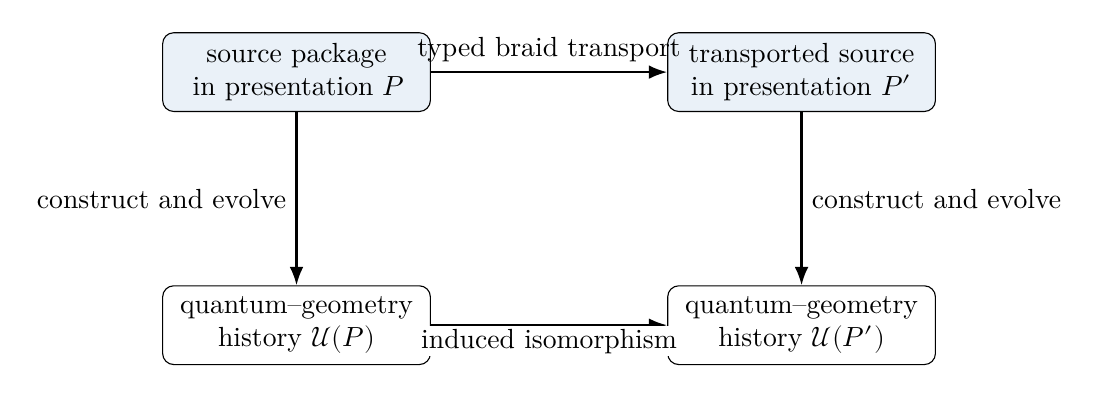
\begin{tikzpicture}[baseline=(current bounding box.center),node distance=22mm and 30mm,>=Latex]
\node[draw,rounded corners,fill=lightblue,align=center,minimum width=34mm,minimum height=10mm] (s) {source package\\in presentation $P$};
\node[draw,rounded corners,fill=lightblue,align=center,right=of s,minimum width=34mm,minimum height=10mm] (sp) {transported source\\in presentation $P'$};
\node[draw,rounded corners,fill=white,align=center,below=of s,minimum width=34mm,minimum height=10mm] (u) {quantum--geometry\\history $\mathcal U(P)$};
\node[draw,rounded corners,fill=white,align=center,below=of sp,minimum width=34mm,minimum height=10mm] (up) {quantum--geometry\\history $\mathcal U(P')$};
\draw[->,thick] (s)--node[above]{typed braid transport}(sp);
\draw[->,thick] (s)--node[left]{construct and evolve}(u);
\draw[->,thick] (sp)--node[right]{construct and evolve}(up);
\draw[->,thick] (u)--node[below,fill=white,inner sep=1pt]{induced isomorphism}(up);
\end{tikzpicture}
\end{equation}
Applying a viewpoint change before constructing the geometry and dynamics gives the same typed result as constructing first and transporting the entire result. State, $H$, cup, clock, $d_C$, soldering, metric, and equations must all move together. Moving only one part defines a different experiment.

This is the precise sense in which no crossing word or matrix presentation is absolute inside the allowed groupoid. A labelled non-Yang--Baxter control fails the full typed equalizer, demonstrating that the relation is not vacuous. Yet the metric-only projection can miss that failure, and the ordinary flip can satisfy the same coherence relation. Braid coherence is therefore sufficient for the declared descent and detected by a faithful full output, while concrete physical uniqueness remains open.

The broader Subjectivity-Intersection programme motivates interpreting an irreducible reciprocal relation as a candidate ``third standpoint'' \cite{watanabe2026ontology,watanabe2026sim}. No such ontology is used in the proof. In particular, mathematical standpoint data are not phenomenal consciousness, and neither light nor a quantum system is called conscious here.

\section{Countermodels, assumptions, and claim boundaries}

\begin{longtable}{>{\raggedright\arraybackslash}p{0.19\linewidth}>{\raggedright\arraybackslash}p{0.34\linewidth}>{\raggedright\arraybackslash}p{0.37\linewidth}}
\toprule
Boundary & Exact finding & Consequence\\
\midrule
\endfirsthead
\toprule
Boundary & Exact finding & Consequence\\
\midrule
\endhead
Section choice & Four time characters are symmetry-related sections of one exact sequence. & The finite $1+3$ screen is built directly on $Q=V_4$ without selecting one.\\
Continuous path & The earlier local generators fail the parameterized Yang--Baxter identity. & The central Braid-Casimir $E_B$ supplies the coherent path.\\
Real continuum & Integer and rational countermodels retain the finite observer--Braid structure without real completeness. & Refinement, Archimedean order, and Dedekind completeness remain explicit axioms.\\
Fixed radix & Triadic refinement is one member of an infinite radix family. & The all-root divisible hull removes radix choice, but finite-division closure and real completion remain assumptions.\\
Endpoint product & The left and right endpoints are distinguished, but only eight of 64 formal product actions satisfy the retained joint consistency rule. & Strong two-clock product independence is unavailable; finite null geometry must be built from the relation quotient.\\
Phase refinement & Integer observer relations preserve insertion, parameterized Yang--Baxter coherence, non-spectator coupling, and signed $R$ limits. & Relation subdivision does not force Floquet roots or completion.\\
Re-entry continuity & The $(z^2,z^3)$ crossing channels recover $z$ exactly, but faithful continuous return of the full orbit is an additional condition. & Geometry inherits $S^1$ continuity conditionally; the real cover still requires history path lifting.\\
Response-quotient descent & Proposition~\ref{prop:descent} proves descent through the declared finite typed congruence. & General measurable or stochastic descent additionally requires quotient measurability and fiber-constant pushforward kernels.\\
Path coherence & Pairwise kernels may each descend while direct and composite transports disagree. & Global path independence is a separate coherence condition, not a consequence of pairwise quotient descent.\\
Multiparty gluing & A Set-colimit may exist while identifying distinct local classes. & Global probes, readouts, and dynamics require overlap compatibility; no multiparty gluing theorem is established here.\\
Promotion uniqueness & The finite response quotient can admit more than one compatible realization. & A canonical promotion requires an extra selector or universal characterization and remains open.\\
Jordan uniqueness & The Jordan product is unique only in the normalized homogeneous bilinear class; $X_c$ gives a rank-ten affine counterfamily. & Rank ten does not globally select one screen.\\
Conservative RP action & A same-six first-order conservative action has an antisymmetric velocity coefficient, but $QJ$ is symmetric positive. & The retained reciprocal principle is Onsager/Lagrange--d'Alembert and remains constitutive.\\
Same-six RP quantization & Six commuting stresses admit no nonzero invariant CCR form in the retained covariance class. & A twelve-dimensional cotangent Gaussian completion is minimal, but its conjugate sector is not yet Braid-derived.\\
Unique Hadamard state & Smooth invariant low-harmonic families preserve the Hadamard class and Braid mark. & State uniqueness from Braid alone is refuted; v0.8 uses one declared target-blind parametric SLE rule.\\
Absolute SLE stress & All finite local Hadamard symbols cancel, and the later line controls the finite-prefix Cauchy kernel, principal ultraviolet mixing, complete $SU(2)$ shell count, and finite-shell matrix remainder. & The global moving-reference inequality and complete typed stress assembly remain open, so the twenty intervals and eight fixed faces are not decided.\\
Fixed target coupling & A nonzero small-$\alpha$ self-consistent constraint branch exists. & The theorem does not reach $\alpha=1$, $\kappa=3/5$ without the complete smooth finite stress.\\
Material current & Exact conservation for all time conflicts with nonzero interaction exchange. & Unit flux is imposed only at creation; later divergence follows the Ward balance.\\
Discrete boosts & A connected real group has no nontrivial continuous action through the discrete lattice automorphism group. & Noncompact boosts require the stated real completion.\\
Rapidity scale & $q=2$ and $q=3$ satisfy the same clock, holonomy, and boost laws. & A crossing does not yet determine a physical rapidity.\\
Four-momentum & The finite Fourier screens fail the commuting translation conditions; bounded $G_1$ cannot be a Lorentz-covariant unbounded $P_0$. & A future model needs an independent unbounded translation carrier coupled nontrivially to the internal Braid holonomy.\\
Nonterminal tower & BIGT yields full matrix algebras at every finite stage, and normalized partial trace supplies an all-finite-stage fixed-$87$ readout. Flip and matched non-YB controls also grow. & Algebraic nonterminality and typed finite-stage readout are established; continuum physics and Braid necessity are not.\\
Infinite completion & The sequential tower completes to the type-$5^\infty$ UHF algebra with unique trace, base expectation, rank-ten readout, continuous state family, and finite-supported Braid automorphisms. & This is a standard algebraic completion and mathematical state continuum, not continuous spacetime, physical time, or infinite-mode QFT.\\
Linear energy--geometry anchor & Symmetry permits rank at most three from the six-dimensional source carrier to the four-dimensional event carrier. & Direct linear compression is closed; nonlinear, operator-system, CP, and GNS routes remain open.\\
Fixed operator geometry & The source-derived four-dimensional operator system is not invariant under the combined generator. & Geometry survives as a moving four-frame, but exact Markov closure needs a nine-dimensional ambient carrier.\\
Low-order metric law & The metric-memory space has dimension $21$ and no common first- or second-order constant-coefficient closure. & Metric alone retains high-order memory; this is not an Einstein-type second-order law.\\
Smooth six-variable reduction & Any smooth faithful invariant state manifold containing the full four-frame has tangent dimension at least nine. & The additional $2+2+1$ directions are independent state information in the declared generator, not eliminable quadratic decorations.\\
Memory-only quadratic stress & The actual geometry response has a nonzero odd linear memory term and a rank-three geometry self-term. & A homogeneous quadratic function of memory alone cannot reproduce the source-canonical response.\\
Pair-history residual & The decomposition is $1+3+2$, with a nonzero irreducible residual two-plane. & The residual cannot be discarded without an operational quotient theorem.\\
Locality and GR & A fixed finite homogeneous Galerkin BIX causal/Ward theorem is conditional on the missing complete conserved ten-tensor callback. & Cutoff-uniform infinite-mode evolution, general $3+1$ Einstein dynamics, and natural gravity remain open.\\
Ontology & The typed relation and viewpoint transport are mathematical. & SIC/O3, subjectivity, and consciousness are interpretations or open bridges, not theorem conclusions.\\
\bottomrule
\end{longtable}

The paper therefore does not establish a unique physical sector, a source-only real continuum, physical seconds or coupling constants, a Braid-selected unique quantum state, general measurable quotient transport, path-independent multiparty gluing, canonical promotion, the absolute matrix-SLE stress, the fixed $\alpha=1$ root, an identification of the five-dimensional memory sector with physical matter or stress-energy, a microscopic Braid origin for RP or the $a$-metric sector, a four-momentum representation, cutoff-uniform or general $3+1$ general relativity, agreement with natural data, or an ontological identity between the mathematical relation and subjectivity. The all-finite-stage fixed-$87$ map is a typed readout, not a tower embedding or a continuum theorem.

\section{Reproducibility and provenance}

The manuscript combines seven versioned lines. The fixed evidential boundaries are:
\begin{itemize}
 \item main stress-reduction line through UB622 at \texttt{f756ba0862ba};
 \item Observer--Braid filtered-observable continuation through OCBFH-020-X1 at \texttt{21a4aba5a07c};
 \item fixed finite-Galerkin causal-evolution applicability audit at \texttt{af50c40e8301};
 \item corrected cutoff-history converter at \texttt{35f87c347e7d}; and
 \item BIGT at \texttt{6f4cc75a93b2}, integrated into the main line by UB495A;
 \item rank-ten cylindrical-limit audit CEML-01 at \texttt{3d4517b8df93}; and
 \item type-$5^\infty$ UHF completion CEML-02-UHF at \texttt{7a9845ac1c19}.
\end{itemize}
Full commit identifiers are fixed in the accompanying manifest. The lines meet only where an explicit dependency record identifies the imported result; branch proximity is not treated as proof. Table~\ref{tab:certificates} is a scoped source-and-certificate ledger, not a full-paper reproduction. A row marked source-recorded means that the manuscript relies on the cited author-native result and its declared assumptions. Only the UB341 row below is accompanied here by a direct reconstruction of the stated measurement map.

\begin{longtable}{@{}p{0.16\linewidth}p{0.58\linewidth}p{0.18\linewidth}@{}}
\caption{Principal source records, executable reconstructions, and scoped negative results in working preprint v0.8.}\label{tab:certificates}\\
\toprule
Records & Certified content & Status\\
\midrule
\endfirsthead
\toprule
Records & Certified content & Status\\
\midrule
\endhead
UB300--340, UB342--387 & Typed source, rank-ten Lorentz carrier, conditional local composition, complete 87D PBM--BIX vector field, interval bounds, and restricted same-source neighborhood; retained at their individual source-record claim ceilings, not reproduced here as one full chain & source-recorded/mixed\\
UB341 & Exact rational $42\times20$ Jacobi measurement map, rank 20, explicit 20-channel inverse with $\|L\|_\infty=13/4$, and 22 redundant consistency channels & reconstructed exact/partial-paper\\
UB388--461 & Raw and signed-sector classification, class-bounded Braid discriminator, finite operational packet, exact orbit isometry, and dual-chart no-go & exact/bounded\\
OB003--014 & Marked coframes, integer word clock, observer groupoid, canonical $\mathbb Z_2$ kernel, $V_4$ quotient, and section-free tetrahedral Lorentz carrier & exact/conditional\\
OB015--017 & Pointwise parity obstruction and logical independence of refinement and real completeness & exact/no-go\\
UB469--472 & Source-Fisher identity, rank-three two-time response, full-coframe character test, and local clock intertwiner & exact\\
UB473--475 & Braid-Casimir parameterized Yang--Baxter path, one-generator C2 system, and section-free quotient Fourier soldering & exact/conditional\\
UB476--479 & Same-$G_1$ rank-ten C5 interface, clock factorization, scoped Jordan classification, and reciprocal density--stress--Ward closure & exact/conditional\\
UB480--486 & Conditional local Weyl net, local CTP/Onsager construction, minimum twelve-dimensional Gaussian CPTP RP completion, and the noisy-RCE automorphism no-go & mixed\\
UB487--499 & Effective curved CTP and compact PBM--BIX response chain, two-anchor ledger, colored-scaling no-go, and conditional two-derivative U4 interval & mixed\\
UB500--594G & Static-response insufficiency, PBM state admissibility, unique Braid-clock state no-go, trace-class Hadamard ball, all-order matrix-block Hadamard theorem, sharp PBM centre tube, exact local $a_6$, and target-blind parametric matrix-SLE family & mixed\\
UB599H/J & Nonzero small-coupling self-consistent constraint branch and cancellation of all finite local Hadamard symbol orders before norms & exact/conditional\\
UB600--605 & All-finite-stage fixed-$87$ typed readout, nonzero marked-boundary response, bilateral re-entry, U3-to-U4 interface closure, finite-prefix four-constraint nondegeneracy, and flux remainder below the fixed face budget & mixed exact/conditional\\
UB606--610 & Abstract sufficient tail/root bounds, global-block type correction, rejection of non-discriminating unsigned Abel envelopes, signed-local finite-prefix packet, and isolation of the missing off-diagonal $C^1$ callback & mixed partial/no-go\\
UB611--622 & Finite covariant coincidence-jet reduction, propagated finite-prefix Wightman Cauchy kernel, actual ultraviolet principal symbol, exact complete $SU(2)$ shell count, dimension-free finite-shell remainder, and reduction to one global reference inequality & exact/partial/open\\
BIGT/UB495A & Nonterminal full-matrix tower from one finite seed, positive and negative controls, and explicit physical-anchor boundary & exact theoretical\\
CEML-01/02-UHF & Rank-ten all-stage cylindrical descent; fixed-amplitude vanishing-mesh no-go; type-$5^\infty$ UHF completion, unique trace, conditional expectation, continuous state family, and finite-supported Braid automorphisms & mixed/open\\
OB018--023 & Equivariant noncompact boost family, pure-Braid rank-three translation, conditional Poincar\'e semidirect closure, residual sector, and bounded-energy no-go & mixed\\
OB024--027 & Non-spectator Floquet--Baxter coupling, primitive operator circle and history cover, phase-root no-go, and conditional A--B--C re-entry continuity theorem & mixed\\
Observer continuation & No-choice path cover, all-root rational repair, endpoint product-independence failure, finite relational $1+3$ null geometry, and rank-four linear-anchor no-go & mixed\\
Observer operator geometry & Source-specific positive four-frame; $4\to6\to8\to9$ minimal closure; order-$21$ metric memory; smooth reduction no-go; canonical $4+5$ balance and block-response laws; memory-only quadratic-stress no-go & mixed exact/no-go\\
OCBFH-019/020-X1 & Filtered source-observable quotient, cup-trace orthogonal representative, and exploratory all-eight-sector retention of rank ten, positivity, Lorentz inertia, and six C5 responses & exact/exploratory\\
Causal applicability & Fixed finite homogeneous Galerkin BIX local-existence and Ward--Bianchi propagation schema; infinite-mode and general $3+1$ boundaries & conditional/open\\
History converter & Abstract cutoff-history Lipschitz converter retained, but direct use of a local Hps germ as a global block kernel rejected; actual no-loss constant and common time remain open & conditional/type correction\\
\bottomrule
\end{longtable}

Standard ingredients are not claimed as original. They include braid groups, Yang--Baxter and Baxterization identities, finite Fourier decomposition, covariance and Fisher metrics, Stone evolution, Lorentz and Poincar\'e representations, Onsager's variational principle, Gaussian quantum dynamical semigroups, Hadamard microlocal structure, states of low energy, Ward balance, and PBM--BIX dynamics. The project-specific synthesis, source realization, section-free soldering, matrix-block SLE extension, BIGT recurrence audit, fixed-finite classifications, and executable certificates were developed in a human-directed process assisted by OpenAI Codex. The author retains responsibility for mathematical verification, interpretation, citations, and release.

\section{Discussion}

The main advance retained from the predecessor is a demonstrable source chain. The Braid-Casimir $G_1$ generates a coherent Yang--Baxter path, finite-time quantum transport, the crossing endpoint, the energy entering the rank-ten screen, and the fixed-finite creation energy. The canonical $V_4$ quotient removes a preferred section, while one reciprocal variational architecture joins density, polarization stress, and Ward exchange.

Version 0.8 changes the status of the finite-source objection in two steps. BIGT establishes a nonterminal tower of finite full-matrix algebras, and Proposition~\ref{prop:stage87} supplies an all-finite-stage, same-law readout into one fixed PBM packet with exact recovery, marked-boundary sensitivity, and bilateral re-entry. Theorem~\ref{thm:uhf} then completes that tower to one infinite-dimensional operator algebra with a mathematical continuum of states while preserving the selected rank-ten readout. This removes the objection that the construction is forced to terminate in a finite carrier. It still does not produce physical spacetime or field modes: the normalized-trace law is fixed rather than uniquely forced, the completion is standard for the declared tensor system, and ordinary flip controls retain part of the finite-stage mechanism.

The quantum-field side has moved beyond Hadamard admissibility. The selected state is one target-blind parametric matrix-SLE family on the frozen $K$ box, and every finite local Hadamard symbol order cancels before interval norms. This establishes the ultraviolet subtraction structure uniformly in the four response directions. It does not determine the smooth finite part: a smooth finite-rank modification can change the renormalized finite stress without changing any local Hadamard coefficient.

The semiclassical constraint problem now has two positive finite results. First, Theorem~\ref{thm:smallcoupling} gives a genuinely state-dependent self-consistent branch for sufficiently small nonzero coupling. Second, the finite $l\le16$ energy/flux prefix has a nondegenerate leading four-constraint Jacobian and a negligible all-time-order flux remainder compared with the fixed face budget. Neither result reaches the fixed target coupling because the global smooth tail remains decisive.

UB608--UB610 prevent two invalid shortcuts. A local Hadamard germ cannot be assigned canonical global harmonic blocks, and a $W-C$ state-gap estimate cannot replace the unknown smooth $C-H_{\rm ps}$ restore. The positive-$\tau$ Abel experiment was correctly non-discriminating because absolute envelopes destroyed signed cancellation. UB611--UB622 then move beyond that first boundary: a finite covariant jet replaces global reconstruction, the actual ultraviolet mixing and complete $SU(2)$ shell arithmetic are controlled, and the finite-shell remainder closes. The outstanding stress obstruction is now one global moving-reference inequality plus typed assembly, rather than an unspecified entire tail.

The causal-evolution result must be read with the same discipline. Once a complete same-scheme conserved ten-tensor is supplied, fixed finite homogeneous Galerkin BIX evolution and Ward--Bianchi propagation have a conditional local theorem. This does not derive Einstein dynamics from Braid or control the infinite-mode limit. A cutoff-uniform history theorem additionally needs a well-typed common stress callback, a no-loss estimate, one common existence time, and convergence of the complete ten-tensor.

The Observer--Braid filtered quotient strengthens the candidate interface without making it unique in nature. After quotienting the low-degree ambiguity and selecting the cup-trace orthogonal representative, all eight finite sectors retain rank ten, positivity, Lorentz inertia, and nonzero C5 response in the exploratory audit. This is a better source-conditioned finite geometry candidate than an arbitrarily chosen Jordan representative, but it still depends on the chosen cup-compatible observation rule and remains exploratory.

Accordingly, two meanings of \emph{unification} remain separate. The effective-U4 target asks whether one explicitly assumed compact homogeneous QFT--geometry model closes at fixed coupling on a controlled interval and later survives a frozen natural-data test. The stronger Braid-origin target additionally requires the continuum, the physical state rule, microscopic RP and metric sectors, and low-energy Einstein dynamics to arise without stagewise fitting. Passing the first programme would not by itself pass the second.

The Subjectivity-Intersection interpretation concerns the commutation of construction with viewpoint transport: changing the marked viewpoint first and then constructing the quantum--geometry system yields the same typed object as constructing first and transporting every component together. This realizes a precise form of non-absolute presentation within the declared groupoid. It does not turn the relation into an observed subject, identify light or quantum systems with consciousness, or prove SIC/O3. Here \emph{subjectivity} denotes the programme's non-objectifiable standpoint primitive and is not equated with phenomenal consciousness.

\section{Conclusion}

Working preprint v0.8 establishes a layered theoretical result. One actual pointed-braid source supports a coherent quantum history, a section-free finite $1+3$ Lorentz carrier, a nonterminal algebra tower, an all-finite-stage fixed-$87$ response history, rank-ten metric response, and conditional reciprocal backreaction. The tower has a type-$5^\infty$ UHF completion with unique trace, compatible base expectation, bounded rank-ten readout, an explicit uncountable compact state family, and finite-supported Braid automorphisms. A minimum Gaussian quantum realization of the effective RP sector, a target-blind parametric all-order Hadamard matrix-SLE family, exact finite-symbol cancellation, and a nonzero small-coupling self-consistent semiclassical constraint branch are constructed under their stated assumptions.

The strongest failures are equally explicit. Algebraic growth, normalized trace, and the finite readout are not uniquely Braid-specific. The Braid clock does not by itself select the SLE rule. The six RP coordinates do not quantize on the same commuting carrier. Left and right endpoints are not product-independent. The current energy carrier has no equivariant rank-four linear quotient onto the event carrier. The moving four-frame is not a closed four-variable dynamics, its metric has no first- or second-order constant-coefficient closure, and faithful smooth Markov reduction below nine dimensions fails. A memory-only homogeneous quadratic stress cannot reproduce the reciprocal block response. Most importantly, cancellation of every local Hadamard symbol does not compute the nonlocal smooth finite stress.

The next effective-U4 step is to prove the remaining global subtract-first reference inequality, complete the twenty total stress intervals, and test all eight fixed $\alpha=1$, $\kappa=3/5$ faces. Only after a root exists can the full conserved ten-tensor time neighborhood, causal coupled evolution, cutoff-uniform field limit, and natural-data protocol be closed. The stronger Braid-origin programme must additionally derive rather than assume the physical continuum, time scale, state principle, microscopic RP and metric sectors, and low-energy Einstein dynamics. Until those gates pass, v0.8 is a mathematically explicit quantum-gravity candidate architecture, not completed quantum gravity, an empirical recovery of general relativity, or an ontological proof.

\section*{Data and code availability}

Version 0.1 is preserved at Zenodo DOI 10.5281/zenodo.22693965 with publication date 10 September 2026. Version 0.2 is preserved at Zenodo DOI 10.5281/zenodo.22700853 with publication date 11 September 2026. Version 0.5 is preserved and verified at Zenodo DOI 10.5281/zenodo.22732287 with publication date 13 September 2026; its public claim boundary ends at UB507. The local predecessor labelled v4.0 is preserved as an unpublished author-review draft. Version 0.6 is preserved locally at commit \texttt{00b8db5a43fa}. Version 0.7 is preserved locally at commit \texttt{346b8a9a22d8}; it retains the main line through UB610 and corrects the quotient, gluing, and promotion scope. Version 0.8 adds the stable UB611--UB622 stress reduction and CEML-01/02-UHF completion identified in the accompanying manifest. No public v0.6 or v0.7 deposit, DOI, journal submission, or external transmission is asserted by this manuscript. Any v0.8 Zenodo DOI is pending exact release approval.

\section*{Competing interests}

The author declares no competing interests.

\section*{Funding}

No external funding is declared for this working preprint.

\section*{AI assistance disclosure}

OpenAI Codex was used under the author's direction for mathematical ideation, derivation assistance, exact-check scripting, audit organization, and drafting. The author retains responsibility for verification, interpretation, citations, and the decision to release this version.

\begin{thebibliography}{99}

\bibitem{artin1947}
E. Artin, ``Theory of braids,'' \emph{Annals of Mathematics} \textbf{48}(1), 101--126 (1947). \href{https://doi.org/10.2307/1969218}{doi:10.2307/1969218}.

\bibitem{yang1967}
C. N. Yang, ``Some exact results for the many-body problem in one dimension with repulsive delta-function interaction,'' \emph{Physical Review Letters} \textbf{19}, 1312--1314 (1967). \href{https://doi.org/10.1103/PhysRevLett.19.1312}{doi:10.1103/PhysRevLett.19.1312}.

\bibitem{lamberadford1997}
L. A. Lambe and D. E. Radford, \emph{Introduction to the Quantum Yang--Baxter Equation and Quantum Groups: An Algebraic Approach}. Springer (1997). \href{https://doi.org/10.1007/978-1-4615-4109-7}{doi:10.1007/978-1-4615-4109-7}.

\bibitem{brunetti2003}
R. Brunetti, K. Fredenhagen, and R. Verch, ``The generally covariant locality principle---a new paradigm for local quantum field theory,'' \emph{Communications in Mathematical Physics} \textbf{237}, 31--68 (2003). \href{https://doi.org/10.1007/s00220-003-0815-7}{doi:10.1007/s00220-003-0815-7}.

\bibitem{hollandswald2001}
S. Hollands and R. M. Wald, ``Local Wick polynomials and time ordered products of quantum fields in curved spacetime,'' \emph{Communications in Mathematical Physics} \textbf{223}, 289--326 (2001). \href{https://doi.org/10.1007/s002200100540}{doi:10.1007/s002200100540}.

\bibitem{choquet2008}
Y. Choquet-Bruhat, \emph{General Relativity and the Einstein Equations}. Oxford University Press (2008). \href{https://doi.org/10.1093/acprof:oso/9780199230723.001.0001}{doi:10.1093/acprof:oso/9780199230723.001.0001}.

\bibitem{pinamontisiemssen2021}
N. Pinamonti and D. Siemssen, ``Existence and uniqueness of solutions of the semiclassical Einstein equation in cosmological models,'' \emph{Annales Henri Poincar\'e} \textbf{23}, 297--329 (2022). \href{https://doi.org/10.1007/s00023-021-01067-8}{doi:10.1007/s00023-021-01067-8}.

\bibitem{meda2026}
P. Meda, ``The semiclassical Einstein equations in cosmological spacetimes,'' \emph{International Journal of Theoretical Physics} \textbf{65}, 137 (2026). \href{https://doi.org/10.1007/s10773-026-06339-9}{doi:10.1007/s10773-026-06339-9}.

\bibitem{olbermann2007}
H. Olbermann, ``States of low energy on Robertson--Walker spacetimes,'' arXiv:0704.2986 (2007). \href{https://arxiv.org/abs/0704.2986}{arXiv:0704.2986}.

\bibitem{banerjeeniedermaier2023}
R. Banerjee and M. Niedermaier, ``States of low energy on Bianchi I spacetimes,'' arXiv:2305.11388 (2023). \href{https://arxiv.org/abs/2305.11388}{arXiv:2305.11388}.

\bibitem{junkerschrohe2001}
W. Junker and E. Schrohe, ``Adiabatic vacuum states on general spacetime manifolds: Definition, construction, and physical properties,'' arXiv:math-ph/0109010 (2001). \href{https://arxiv.org/abs/math-ph/0109010}{arXiv:math-ph/0109010}.

\bibitem{gerardetal2016}
C. G\'erard, O. Oulghazi, and M. Wrochna, ``Hadamard states for the Klein--Gordon equation on Lorentzian manifolds of bounded geometry,'' arXiv:1602.00930 (2016). \href{https://arxiv.org/abs/1602.00930}{arXiv:1602.00930}.

\bibitem{brattellirobinson1997}
O. Bratteli and D. W. Robinson, \emph{Operator Algebras and Quantum Statistical Mechanics 2: Equilibrium States, Models in Quantum Statistical Mechanics}, 2nd ed., Springer (1997). \href{https://doi.org/10.1007/978-3-662-03444-6}{doi:10.1007/978-3-662-03444-6}.

\bibitem{watanabe2026braid}
S. Watanabe, \emph{Subjectivity-Intersection Mathematics: All-Orders Intersection Consistency and Compositional Objectivity from Pointed Unitary Braids}, version 1.0, Zenodo (2026). \href{https://doi.org/10.5281/zenodo.22166167}{doi:10.5281/zenodo.22166167}.

\bibitem{watanabe2026ontology}
S. Watanabe, \emph{Subjectivity Intersection Ontology: A Comparative Ontological Framework for Third Subjectivity}, version 1.0.0, Zenodo (2026). \href{https://doi.org/10.5281/zenodo.21641878}{doi:10.5281/zenodo.21641878}.

\bibitem{watanabe2026sim}
S. Watanabe, \emph{Subjectivity-Intersection Mathematics Public Working Preprint v4.2 Draft}, Zenodo (2026). \href{https://doi.org/10.5281/zenodo.21909933}{doi:10.5281/zenodo.21909933}.

\end{thebibliography}

\end{document}
